% ------------------------------------------------------------------------
% A Latex "template" for CMP MSc Dissertation. 
% 
%
% Please read the brief Instructions (Instrucrtions.tex) below and in sample files 
% to learn how to use this option in this template.
%
%
% Notes and sample files:
% "acronymNotes.tex": brief introduction on how to make a LOA. 
% "acronyms.tex": a sample file where you define abbreviations.
%  
%   
% Brief Instructions
%#### 
%% Preparations: 
% (i)  Download the zipped Latex templat file into your disk or your university's home space on U disk,
% (ii) Unzip all the fiels into your working folder, such as \Dissertation. 
% (ii) Change/replace/fill few places in this "DissertationTemplate.tex" file to suit your need:
% 		such as, Your course, Year, Dissertation title, your name, markers, etc.
%
%% Then you can follow teh following instructions(not necessarily in that order) to write your dissertation. 
%   
%% 1. Write your abstract in a separate tex file and name it as ABS.tex
%% 2. Write your acknowledgement in a separate tex file and name it as ACK.tex  
%    Note: Both ABS.tex and ACK.tex files are already included in the style file. 
%
%% 3. wirte each chapter in a separate tex file and name e.g. Ch1, Ch2, etc. 
% and then use "include" to inlcude them as shown in this example.
% 
%#### 
% If you wish to produce a list of abbreviations/acronyms 
% that are used in your dissertation, you must read notes 4-7 below. 
%
%% 4. Define abbreviations or acronyms
% 	you can use the given sample file "acronyms.tex" 
% 	to define your abbreviations or acronyms, and 
% 	some examples are already defined in that file.
% 	After you have defined them, (you can add any new items anytime you like), 
% 	save it in the same folder as this "DissertationSample1.tex"
% 	as it is included by using "include{acronyms}" in this file later.
% 	Note: if you use any other file name, change it in "\inlcude{yourFilename}. 
%
%% 5. Using the defined abbreviations/acrynoms
%   In file "acronymNotes.tex", I give some notes and few examples 
%   to explain and show how to use defined acrynoms in your tex file.  
%
%% 6. Generate a List of Abbreviations(LOA)
%  You must issue command "Makeglossaries" to produce few more auxiliary files 
%   e.g. xxxx.acr, and/or .glo, and/or .gls, etc. in order to produce LOA 
%   so, is you use TexStudio, Click "Tools" and choose "Makeglossaries"
%
%% 7. Don't want to have a list of Abbreviations
%  use command "\nolistofabbs", by uncomment it in later part  
%  then LOA will not be generated and not appear in the TOC. 
%  note: you may have to run "Build and View" twice to get the intended result.
%        first run to remove/get the acutal list of abbreviation
%		 second run to remove/get the list appearing on TOC.   
% 
%% 8. Using footnote. (% wjw, added this note on 11/09/2015)
%	If you want to use footnotes in any chapters of your dissertation, 
%	you can use command \footnote{your footnote text} in where you want.
% 	The footnotes are numbered automatically and continuously within a CHAPTER.   
%   
%% 9. Citation styles:
%   Add package "natbib" onto the preamble of your dissertation file 
%   if it is not added, using "\usepackage{natbib}"
%   (i) Use Command "\citep{...}" to produce the styyle: (Authors, year)
%   (ii) Use Command "\citet{...}" to produce the style: Authers (year)
%
%
% Disclaimer: This template is provided as it is. 
% You are welcome to try it, 
% but Dr. Wang won't be held responsible for any problems it has or causes.
% 
%
% ------------------------------------------------------------------------
\documentclass[a4paper,12pt]{report}
\usepackage[centertags]{amsmath}
\usepackage{amsfonts}
\usepackage{amssymb}
\usepackage{amsthm}
\usepackage{newlfont}
\usepackage{graphicx}
\usepackage{graphicx}
\usepackage{float}
\usepackage{url}
\usepackage[page,toc,titletoc,title]{appendix}
\usepackage{natbib} % by wjw 22/11/2016 to replace apalike package
%\usepackage{pdfsync} %PDF Forward Search

\usepackage[acronym]{glossaries} % added by wjw on 05/08/15
%\usepackage{datetime}

\usepackage{CMPDissertation3a} % CMP Dissertation Style

\usepackage{XTocinc} % Include Table of Contents as the first entry in TOC

\usepackage{setspace}  % added by wj on 11/09/15
% Note: this makes the body text in chapters are double spaced 
% and text in table are single spaced.
% If you want to have a double space in tables, commented it out. 


%\usepackage[active]{srcltx}  %SRC Specials for DVI search




% Fuzz -------------------------------------------------------------------
\hfuzz2pt % Don't bother to report over-full boxes if over-edge is < 2pt
% Line spacing -----------------------------------------------------------
\newlength{\defbaselineskip}
\setlength{\defbaselineskip}{\baselineskip}
\newcommand{\setlinespacing}[1]%
           {\setlength{\baselineskip}{#1 \defbaselineskip}}
% As the package setspace is included above, which define linespacing, 
% the following newcommands for double/single spacing become redeundant, 
% hence they were commentted out. wj 11/09/2015   
%\newcommand{\doublespacing}{\setlength{\baselineskip}{2.0 \defbaselineskip}}
%\newcommand{\singlespacing}{\setlength{\baselineskip}{\defbaselineskip}}

% MATH -------------------------------------------------------------------
\newcommand{\A}{{\cal A}}
\newcommand{\h}{{\cal H}}
\newcommand{\s}{{\cal S}}
\newcommand{\W}{{\cal W}}
\newcommand{\BH}{\mathbf B(\cal H)}
\newcommand{\KH}{\cal  K(\cal H)}
\newcommand{\Real}{\mathbb R}
\newcommand{\Complex}{\mathbb C}
\newcommand{\Field}{\mathbb F}
\newcommand{\RPlus}{[0,\infty)}
%
\newcommand{\norm}[1]{\left\Vert#1\right\Vert}
\newcommand{\essnorm}[1]{\norm{#1}_{\text{\rm\normalshape ess}}}
\newcommand{\abs}[1]{\left\vert#1\right\vert}
\newcommand{\set}[1]{\left\{#1\right\}}
\newcommand{\seq}[1]{\left<#1\right>}
\newcommand{\eps}{\varepsilon}
\newcommand{\To}{\longrightarrow}
\newcommand{\RE}{\operatorname{Re}}
\newcommand{\IM}{\operatorname{Im}}
\newcommand{\Poly}{{\cal{P}}(E)}
\newcommand{\EssD}{{\cal{D}}}
% THEOREMS ---------------------------------------------------------------
\theoremstyle{plain}
\newtheorem{thm}{Theorem}[section]
\newtheorem{cor}[thm]{Corollary}
\newtheorem{lem}[thm]{Lemma}
\newtheorem{prop}[thm]{Proposition}

\theoremstyle{definition}
\newtheorem{defn}{Definition}[section]
%
\theoremstyle{remark}
\newtheorem{rem}{Remark}[section]
%
\numberwithin{equation}{section}
\renewcommand{\theequation}{\thesection.\arabic{equation}}
%%% ----------------------------------------------------------------------
\setlength{\tclineskip}{1.05\baselineskip}
%%% ----------------------------------------------------------------------
%\nobib
%\draft
%\nofront

%\permissionfalse

\dedicate{}

%\nolistoftables
%\nolistoffigures
% if you don't want to have a list of Abbreviations
% decomment the followling command
%\nolistofabbs

% This is an MSc dissertation
\msc

% if this is for  PhD thesis
%\phd

\university{The University of East Anglia}
\school{Computing Sciences}

%%%%%% You need to change/fill few things from here %%%%%%

%#### CHOOSE OR INSERT YOUR MSC COURSE TITLE BELOW #####
% by commentting in your course from the liste befow.

%\course{Advanced Computing Science}
\course{Computing Science}
%\course{Games Development}
%\course{Information Systems}
%\course{Data Mining and Knowledge Discovery}
%\course{Computational Biology}

%####-------------------------------
% change the year and month to the current ones
%\monthyeardate\today

\copyrightyear{2019}
\submitdate{August, 2019} % Change to your submission date
%\submitdate{\date{today}}
\studyyears{2018}{2019} % insert your start and finish years of your course.
%\convocation{August}{2017}

% ------------------------------------------------------------------------
% #### Insert the title of your dissertation below.#####
\title{The Impact of Previous User Knowledge on the Concurrent Think-aloud Methodology}

% #### Insert your full name below.#####
\author{George Bennett}

%#### insert your supervisor's name below #####
\supervisor{ Dr. Pam Mayhew}

%#### insert the name of your markers if you know them #####
\firstmarker{Marker 1: Dr. Pam Mayhew}
\secondmarker{Marker 2: Dr. Antony Jackson}
\examiner{Checker/Moderator}
\organiser{Dr. Wenjia Wang}

% inlcude a tex file here, e.g. acronyms.tex, 
% where you have defined your acronyms and abbreviations.   
%####
% File name: acronyms.tex
% purpose: a sample file that is used to define abbreviations, acronyms, glossary.
% Created on 05/08/2015, by Wenjia Wang

%#### Notes:
% In this file, you can define all the abbreviations you wish to use in your text.

% 1. Use command "\newacronym" to define an abbreviation/acronym 
% format: \newacronym{label}{name}{description}
% for example:  
\newacronym{cmp}{CMP}{School of Computing Sciences}
\newacronym{uea}{UEA}{University of East Anglia}
\newacronym{loa}{LOA}{List of Abbreviations}

% 2. use command "\gls{label}" or "\Gls{label}" to cite a defined acronym in your .tex file 
% for example: \gls{UEA}
% when used it in the first time, it will produce: University of East Anglia(UEA)
% when used after the 1st time, it will produce: UEA    

% Some more examples defined here.

\newacronym{api}{API}{Application Programming Interface}
\newacronym{uml}{UML}{Unified Modelling Language}
\newacronym{kdd}{KDD}{Knowledge Discovery form Database}
\newacronym{svm}{SVM}{Support Vector Machine}


\newacronym{ta}{TA}{Think Aloud}
\newacronym{cta}{CTA}{Concurrent Think Aloud}
\newacronym{rta}{RTA}{Retrospective Think Aloud}
\newacronym{hci}{HCI}{Human Computer Interaction}
\newacronym{ux}{UX}{User Experience}
\newacronym{ui}{UI}{User Interface}
\newacronym{gdpr}{GDPR}{General Data Protection Regulation}

\newacronym{bpm}{BPM}{Big Picture Mode}
\newacronym{nil}{NIL}{New Invite Link}

% or use the following command to define a glossary term %"\newglossaryentry{label}{name={<name>}, description={<describing blahh blah}}
% e.g

\newglossaryentry{apple}
{
	name={apple}, 
	description={is a kind of sweet fruit}
}
\newglossaryentry{latex}
{
	name=Latex,
	description={is a mark-up text-editing language specially   
		for writing scientific documents}
}

\makeglossaries


%------------------------------------------------------------------------
\begin{document}
{
\typeout{:?000000000} % Don't bother with over/under-full boxes
\beforepreface
\typeout{:?111111111} % Process All Errors from Here on
}

\afterpreface
\def\baselinestretch{1}
\setlinespacing{1.66}

%--------------------------------------------------------------------

%------------------------------------------------------------------------

% ##### Include each chapter in order below #####

%% S sample tex to show to how use the defined abbreviations/acronums in file "acronym.tex"
% 
% ------------------------------------------------------------------
\def\baselinestretch{1}

\chapter{Notes on how to use the Latex Dissertation template}

\def\baselinestretch{1.66}

%%% ----------------------------------------------------------------------
This LATEX template was created by Dr. Wenjia Wang\footnote{Created in 2005 based on a thesis style file from Stanford University. 

Previous versions: created in 2005 (v0), updated in 2010(v1) and 2012(v1.1).  
	Major Revision on 06/08/2015-17/08/2015(v2): Added the function of generating the list of Abbreviations (you must follow the instructions carefully and exactly in order to produce a list of Abbreviations). 
	Major revision on 22/11/2016(v3), added notes for how to use the Template.   
	Latest update on 15/04/2019: Just updated the Instruction notes.  }
with aim of helping Master students at the \gls{cmp}, the \gls{uea}, to write their dissertation with Latex.  %It has been developed and evolved from several early versions based on various sources as indicated in the Sample file. 
% by adding an option of generating a list of Abbreviations. 

This section gives some brief instructions on how to use it and you should read it carefully before attempting it.

NOTE: you should use $TexStudio$ as your text editor and Latex compiler to make sure this Latex  Template working properly, although it may work with other text editors.
 
 
Please let me know if you find any bugs or problems, although I may not have time to resolve them in time.
 
 
\section{How to use this Latex Template}

 %Read the brief notes below and in sample files to learn how to use this option in this template.  
  
 
 Brief Instructions:
 
\subsection{Preparations: P1 to P4} 
 
P1. Download the template package from the blackboard of Dissertation Module and
Unzipped it to an intended working folder on your U drive, e.g. Dissertation.    

P2. Start TexStudio and open ``DissertationTemplate4.tex" 

Note: it is a tex file that (1) uses, i.e. includes all the other files, such as Abstract, Acknowledgement, and chapter files, which are written or edited separately with Latex, 
(2) generates a pdf file of your dissertation as a whole.         
 
P3. Change/replace/fill few places in this file to suit your need:
 		such as, Your course, Year, Dissertation title, your name, markers, etc.
 		
P4. Save it with your new file name, e.g. ``Wang\_Dissertation2019.tex" 


\subsection{Work on each latex file}
		
Then following steps below to work on each file to write your dissertation.    

 1. Write your abstract in a separate tex file and name it as Abstract.tex
 2. Write your acknowledgement in a separate tex file and name it as Acknowledgement.tex  
    Note: Both Abstract.tex and Acknowledgement.tex files are already included in the style file.
    So you must not change their names but only the contents.    

 3. write each chapter in a separate tex file and name them as, e.g. Ch1, Ch2, etc. 
 and then use ''$\backslash$include\{...\}" to include them as shown in this example.
 
New notes added on 06/08/2015

4. If you wish to produce a list of abbreviations/acronyms 
 that are used in your dissertation, you must read notes below. 

% 4. Define abbreviations or acronyms
% 	you can use the given sample file "acronyms.tex" 
% 	to define your abbreviations or acronyms, and 
% 	some examples are already defined in that file.
% 	After you have defined them, (you can add any new items anytime you like), 
% 	save it in the same folder as this "DissertationSample1.tex"
% 	as it is included by using "include{acronyms}" in this file later.
% 	Note: if you use any other file name, change it in "inlcude{yourFilename}". 
%
% 5. Using the defined abbreviations/acronyms
% 
%   In file "acronymNotes.tex", I give some notes and few examples 
%   to explain and show how to use defined acrynoms in your tex file.  
%
% 6. Generate a List of Abbreviations(LOA)
% 
%  You must issue command "Makeglossaries" to produce few more auxiliary files 
%   e.g. xxxx.acr, and/or .glo, and/or .gls, etc. in order to produce LOA 
%   so, is you use TexStudio, Click "Tools" and choose "Makeglossaries"
%
% 7. Don't want to have a list of Abbreviations
% 
% Use command $\backslash$nolistofabbs, by uncomment it in later part  
%  then LOA will not be generated and not appear in the TOC. 
%  note: you may have to run "Build and View" twice to get the intended result.
%        first run to remove/get the acutal list of abbreviation
%		 second run to remove/get the list appearing on TOC.   
% 
5. Using footnote. (wjw added this note on 11/09/2015)
 
 If you want to use footnotes in any chapters of your dissertation, 
	you can use command $\backslash$foodnote\{foodnote text\} in where you want, for example 
	\footnote{your footnote text: If you want to generate a list of Abbreviations, you must follow the instructions given here carefully and exactly, particularly using Command "Makeglossaries" in "Tools" before Compiling.} 
	
The footnotes are numbered automatically and continuously within a CHAPTER. 

\section {Making Citations and Citation Styles}

You are  required to use the Harvard style for citing references.

Specifically, there are two sub-styles to be used in different situations.

1. Use command $\backslash citep\{...\}$. 

If the authors of a reference are NOT part of your sentence, e.g. ``A study (Wang, 2008) has been done to investigate the influence of some factors on the accuracy of an ensemble.", then use $\backslash$citep\{...\} in your Latex file, such as ``A study $\backslash$citep\{Wang08\} has been done...", it then produces the text as: 
``A study \citep{Wang08} has been done......"

2 Use command $\backslash citet\{...\}$.

If the authors of a reference are part of your sentence, e.g. ``Wang (2008) studied the factors that can affect the performance of a machine learning ensemble.", then use $\backslash$citet\{Wang08\} studied ... . It then produces the text as: `` \citet{Wang08} studied ......" 
  
You can press function key ``F8" in TexStudio to compile bibliography, i.e. to pull all the cited references out from your Bibtex file and generate a bib file. The message shows if there is any error in this process.       

\section{Creating Equations}

You can write an equation by using $\backslash$begin\{equation\} write equation here $\backslash$ end\{equation\}. For example, 

\begin{equation}
y = a + b_1x_1 + b_2x_2
\end{equation}

If your equation is too long for a single line, instead of using the above environment,  
use ``$\backslash$begin\{align\}" command to align an equation of multiple lines at a specified point. 
Use $\backslash\backslash$ to specify a line break, and \& to indicate where  the lines should be aligned. 

For example, the following equation is aligned at ``=". 

\begin{align}
f(x) &= (x+a)(x+b) \nonumber \\
&= x^2 + (a+b)x + ab
\end{align}

The following equation is aligned at the left brace.  

\begin{align}
f(x) &= \pi \left\{ a + b_1x_1 + b_2x_2+ b_3x_3^4 + b_4{x_4}^3 + b_5x_5^2 \right.\nonumber\\
&\qquad \left. {} + b_6x_6^5 + b_7x_7^2+ b_8x_8^3 + b_9{x_9}^3 \right\}
\end{align}  

Note: ``\emph{\{align\}}" must not be nested within ``\emph{\{equation\}}", it replaces ``\emph{\{equation\}}".

If you do not want to automatically number an equation, use  \{equation*\} or  \{align*\}. For example, the following equation will not be numbered.   

\begin{equation*}
y = a + b_1x_1 + b_2x_2^2 + b_3x_3^3
\end{equation*}

\section{How to define and generate a list of Abbreviations}

% text for testing abbreviations
In the first paragraph I will show you how to use the acronyms defined in file ``acronyms.tex", which will be then listed in the \gls{loa} if they are used in your text.

\subsection{Define abbreviations/acronyms}

( Notes and sample files:

 "acronymNotes.tex": brief introduction on how to make a LOA. 
 
 "acronyms.tex": a sample file where you define abbreviations.
)

To define an abbreviation or acronym, open ``acronym.tex" file in any text editor, e.g. TeXstudio, you can see some abbreviations (or acronyms) already defined in it.

You can simple use teh following command \emph{newacronym} to define an abbreviation/acronym 
in the format: $\backslash$newacronym\{label\}\{name\}\{description\}

For example:  
% the acutal command: \newacronym{uk}{UK}{The United Kingdoms} 
% but to show it in the complied text, 
$\backslash$newacronym\{api\}\{API\}\{Application Programming Interface\}\} 
 
\subsection{Use the defined abbreviations/Acronyms}

You can use $\backslash$gls, or  $\backslash$Gls, Capital, to insert the abbreviation to any where you want in your tex file. 
Or use $\backslash$glspl, or  $\backslash$Glspl for using their plural forms. 

In the first time you use it, it will produce the full text of the abbreviation, followed by its abbreviation in (). After that, it will only produce the abbreviation.   

For example,      
$\backslash$Gls\{api\} 
%\Gls{api}
 will be shown as \gls{api}, i.e. 'Application Programming Interface (API)' 
(without the quotation marks), 
and will add a linked page number to where it uis used, e.g. '1' in this case, and will be shown in the \gls{loa}. 

After that, $\backslash$Gls\{api\} will produce only the abbreviation, i.e. \gls{api}.

\gls{uml}, \gls{svm}, \gls{kdd} are some other abbreviation examples I defined in ''acrynom.tex" file. Their plural format can be produced by using command: $\backslash$glspl\{\}.
 e.g.  $\backslash$glspl\{uml\}, $\backslash$glspl\{svm\},  $\backslash$glspl\{kdd\}, which produce:   
% the acutal commands are as follows: 
    \glspl{uml}, \glspl{svm}, \glspl{kdd}.  


\section{Compiling/Building your tex file}

After you have defined your abbreviations or acronyms in file ``acronyms.tex", and use some of them in your text file of other Chapters, such as in this note file, by using the commands given above, you need to compile and build your integrating tex file (e.g. DissertationSample1.tex) to produce the intended files, e.g. pdf file, with following steps in TeXstudio. 

1. Run ``Compile" or ``Build/View" by clicking their icon.
(note: you may see a pdf file with your text, but it won't have the list of abbreviations.)

2. Run ``Makeglossaries": 
Click ``Tools" and then ``Commands", and choose ``Makeglossaries" to run it. 

Ignore any warning message.

Note: whenever you make any new entry to your ``acronym.tex" file, and/or use any abbreviation/acronym in your other tex file, you must do this step to update your generated .gls file.   

3. Run ``Build and View" again. 
This time the pdf file should contain the actual list of abbreviations after the list of Figures and teh title appears in the Table of Content(TOC).
          

Please note:

(1) Only the used acronyms will appear in the list of Abbreviations.

(2) notice the difference in using "gls{}" and "glspl{}" 

%%%-----------------

%\def\baselinestretch{1.66}
%\medskip

%%% ----------------------------------------------------------------------
 % you can edit this out in your file, but keep the tex and pdf files 
%% ------------------------------------------------------------------------
% -*-TeX-*- -*-Hard-*- Smart Wrapping
% ------------------------------------------------------------------------
\def\baselinestretch{1}

\chapter{The Space of Lomonosov Functions}

\def\baselinestretch{1.66}

%%% ----------------------------------------------------------------------

This chapter gives a constructive proof of an abstract
approximation theorem, inspired by the celebrated result of
V.I.\,Lomonosov~\citep{Lom73}. 

\citet{AAB95} gave an alternative proof of some recent characterizations of the
invariant subspace problem. We also
establish density of non--cyclic vectors for certain convex
sets of compact quasinilpotent operators, and conclude with a
related open question. In Chapter 2 we extend the techniques
introduced in this chapter to non--compact operators acting on
a Hilbert space.

\smallskip

%%% ----------------------------------------------------------------------
\goodbreak
\section{Introduction}

\citet{Lom91} conjectured that the
adjoint of a bounded operator on a Banach space has a
non--trivial closed invariant subspace. In view of the known
examples of operators without an invariant subspace
\citep{Enf87,Rea85}, this is the strongest version of the
invariant subspace problem that can possibly have an
affirmative answer. In particular, if the Lomonosov conjecture
is true, then every operator on a reflexive Banach space has a
non--trivial invariant subspace(as shown in Figure \ref{fig1}).

\begin{figure}
\centering
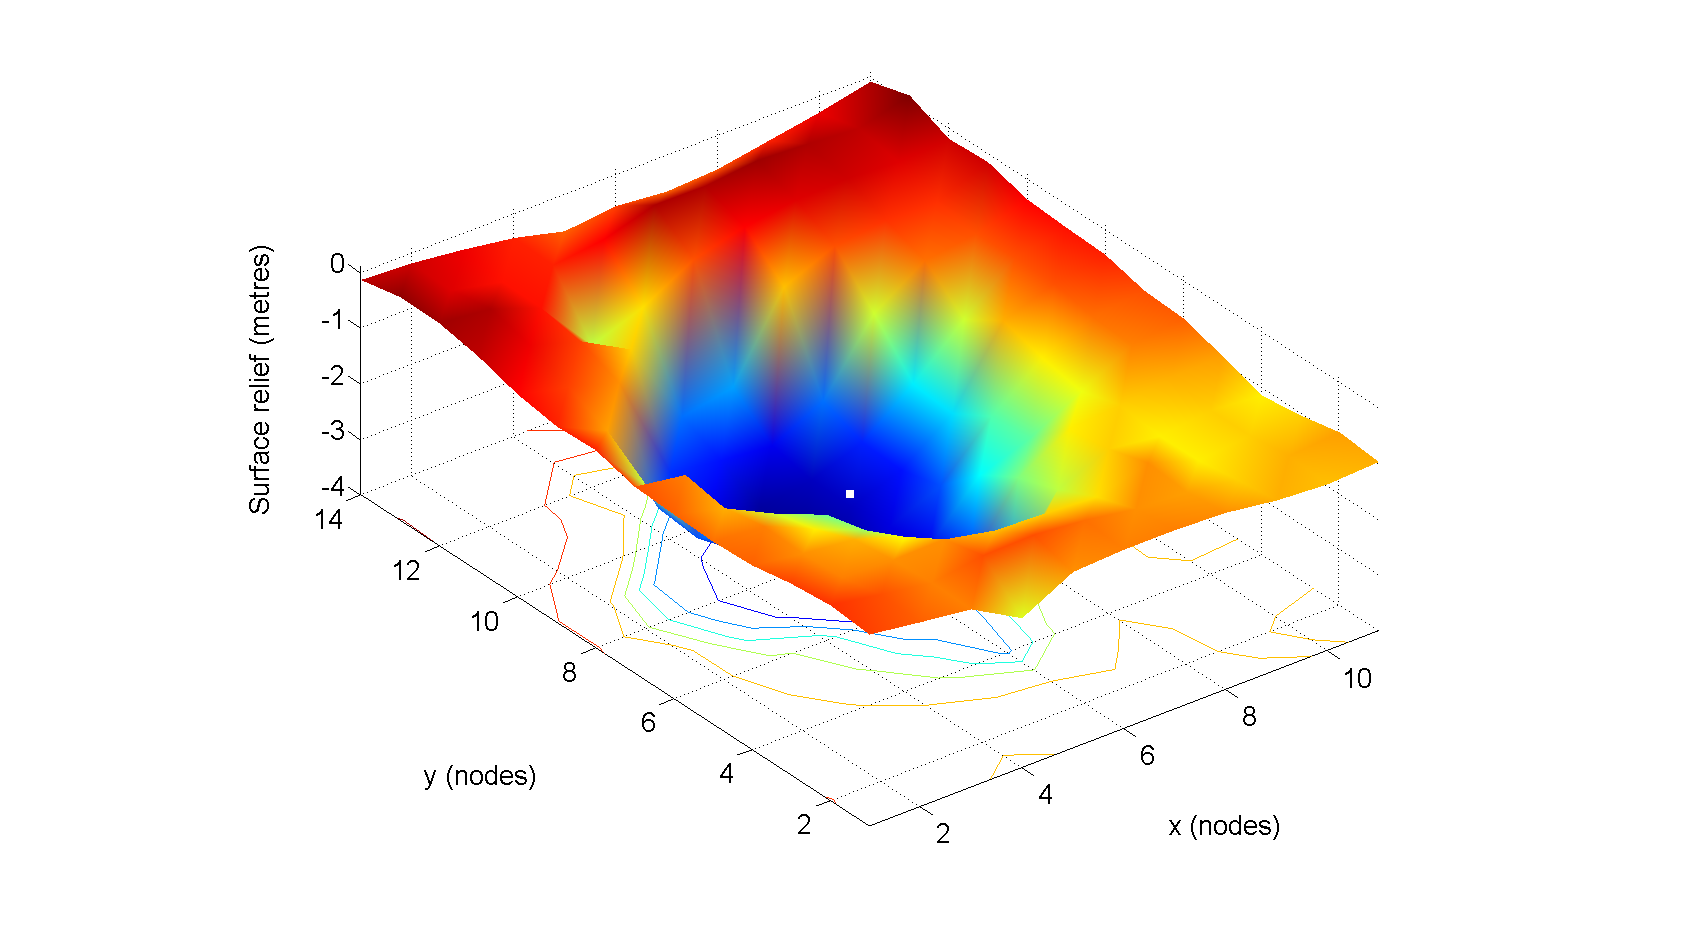
\includegraphics[scale=0.25]{fig1}
\caption{A figure sample that is not associated with the text.}
\label{fig1}
\end{figure}

\bigskip
\goodbreak

Considering the strong influence of Lomonosov's results on the
theory of invariant subspaces, it is not surprising that both
the conjecture and the techniques developed in the interesting
paper \citep{Lom91} received further attention. L.~de~Branges
used this result to obtain a characterization of the invariant
subspace problem in terms of density of certain functions. This
stimulated another characterization of the invariant subspace
problem given by Y.A.~Abramovich, C.D.~Aliprantis, and
O.~Burkinshaw ~in~\citep{AAB95}. Section~1.4 presents a more
detailed account of this work.

We take a slightly different approach. First we give a
constructive proof of the approximation theorem, inspired by
the well known Lomonosov construction used in
\citep{Lom73,RR73}. This theorem is then applied to give an
alternative proof of the main result in \citep{AAB95}. Our proof
applies to both real and complex Banach spaces, while the
original result was established for complex Banach spaces only.
The alternative proof somehow explains the role of compact
operators that appear in the characterizations of the invariant
subspace problem~\citep{AAB95}.

\medskip

\begin{table}
\caption{A sample Table}
\begin{center}
    \begin{tabular}{ | l | l | l | p{5cm} |}
    \hline
    Day & Min Temp & Max Temp & Summary \\ \hline
    Monday & 11C & 22C & A clear day with lots of sunshine.  
    However, the strong breeze will bring down the temperatures. \\ \hline
    Tuesday & 9C & 19C & Cloudy with rain, across many northern regions. Clear spells
    across most of Scotland and Northern Ireland,
    but rain reaching the far northwest. \\ \hline
    Wednesday & 10C & 21C & Rain will still linger for the morning.
    Conditions will improve by early afternoon and continue
    throughout the evening. \\
    \hline
    \end{tabular}
\end{center}
\label{tbl1}
\end{table}

One may notice that the weak*--compactness of the unit ball in
dual Banach spaces plays an important role in
\citep{AAB95,dB59,dB93,Lom91}, as well as in the applications
given in this chapter. In other words, if the Lomonosov
conjecture is true, then the compactness of the unit ball, with
respect to the weak* topology, is likely to be an important
ingredient of its proof.

\smallskip

In the last section we put this observation to the test. A
straightforward application of the approximation theorem
obtained in Section~1.3, together with the Schauder--Tychonoff
Fixed Point Theorem, yields density of non--cyclic vectors for
the dual of a convex set of compact quasinilpotent operators.
We end with the open problem of obtaining a similar result for
the original set, rather than its dual.

\bigskip

This work is more or less self--contained and the notation and
terminology used in it is (supposed to be) standard. However,
here are a few conventions that hold throughout this chapter:


\bigskip

%%% ----------------------------------------------------------------------
\goodbreak

\def\baselinestretch{1.1}

\section{Reflexive Topological Spaces and Continuous Indicator Functions}

This section introduces some topological preliminaries that
lead to a fairly general treatment of the approximation theory
in the next section, where an important role is played by the
partition of unity and the ``continuous indicator functions''
associated with a basis for the topology on a compact domain of
certain functions. The existence of continuous indicator
functions can be characterized by a purely topological property
of the underlying space, which is defined as ``reflexivity'' of
the topological space. In this section we introduce both
concepts and establish the connection between them.

\def\baselinestretch{1.66}

\begin{defn}
Let $S=(S,\tau)$ be a topological space and denote by
$C(S,\Real)$ the space of all continuous real--valued functions
on $S$. A topological space $S$ is called {\em reflexive} if
the topology $\tau$ coincides with the weakest topology
$\tau_w$ on $S$ for which all the functions in $C(S,\Real)$ are
continuous.
\end{defn}

\begin{rem}
The reflexivity of topological spaces is not to be confused
with the corresponding concept of the reflexivity of Banach
spaces. Indeed, we conclude this section by showing that every
subset of a locally convex space is reflexive.
\end{rem}

\begin{prop}
Reflexivity is a hereditary property; \, i.e. a subspace $S$ of
a reflexive topological space $X$ is reflexive with the
relative topology.
\end{prop}

\begin{proof}
Consider the restrictions of the functions in $C(X,\Real)$ to
the subset $S$, and observe that they induce the relative
topology on $S$, whenever $X$ is reflexive.
\end{proof}

\begin{defn}
Suppose $U$ is an open subset of a topological space $S$. A
continuous function $\Gamma\colon S \To \RPlus$ is called a
{\em continuous indicator function} of $U$ in $S$ if
\[ U = \set{s\in S \,\,|\,\,\, \Gamma(s) > 0}.  \]
\end{defn}

\begin{rem}
If $X$ is a metric space then every open ball
\[ U=U(x_0,r)=\set{x\in X \,\,|\,\,\, d(x,x_0) < r}, \]
admits a continuous indicator function
$\Gamma_U\colon{X}\To\RPlus$, defined by
\[ \Gamma_U(x) = \max\set{0, \, r - d(x,x_0) }. \]
Furthermore, suppose $f \in C(S,X)$. Then the open set
$V=f^{-1}(U)\subset S$ ``inherits'' an indicator function from
$U$ by setting: $\Gamma_V(s)=\Gamma_U(f(s))$.
\end{rem}

\smallskip
\goodbreak


%%% ----------------------------------------------------------------------
\goodbreak
\section{Lomonosov Functions}

The proof of the celebrated result of V.I. Lomonosov
\citep{Lom73,RR73} was based on the ingenious idea of defining a
continuous function with compact domain in a Banach space,
assuming that certain local conditions are met. In this section
we generalize this idea in the form of an approximation
theorem. Since our construction was greatly inspired by the
proof of Lomonosov's Lemma~\citep{Lom73,RR73}, we suggest the
following definition.

\begin{defn}
Let $\A \subset C(S,X)$ be a subset of the space of continuous
functions from a topological space $S$ to a locally convex
space $X$. The convex subset $\cal{L}(\A) \subset C(S,X)$,
defined by
\[ \cal{L}(\A) = \set{ \sum_{k=1}^n \alpha_k A_k \,\,|\,\,\, A_k\in\A,
   \alpha_k\in C(S,[0,1]) \text{ and } \sum_{k=1}^n\alpha_k \equiv 1;
   \,\, n < \infty}. \]

is called the {\em Lomonosov space} associated with the set
$\A$, and a function $\Lambda \in \cal{L}(\A)$ is called a {\em
Lomonosov function}.
\end{defn}

\begin{equation}
y = a + b_1x_1 + b_2x_2
\end{equation}

\medskip

Recall that the {\em uniform topology} on $C(S,X)$ is induced
by the topology on a linear space $X$. If $\cal{B}$ is a local
basis for the topology on $X$ then the sets
\[ \widehat{U}=\set{f\in C(S,X) \,\,|\,\,\, f(S)\subset U\in\cal{B}} \]
define a local basis for the uniform topology on $C(S,X)$. If
$X$ is a locally convex space then so is $C(S,X)$. In
particular, if $X$ is a Banach space then $C(S,X)$ with the
uniform topology is a Banach space, as well.

\medskip

We are now ready to give a construction of the Lomonosov
function that uniformly approximates a continuous function
within a given neighborhood.


%%% ----------------------------------------------------------------------
\goodbreak

\def\baselinestretch{1.1}

\section{Subspace Problem}

We introduce some basic concepts and notation that is
consistent with \citep{AAB95}. However, for more details and
further references on the {\em invariant subspace problem}, the
reader is advised to consult the nicely written and
comprehensible original~\citep{AAB95}.

\def\baselinestretch{1.66}
\medskip


%%% ----------------------------------------------------------------------

\draft
\chapter{Project Introduction}
\section{Project Overview}
This chapter provides an overview to my project. Firstly defining usability in the context of \gls{hci} and the \gls{ta} methodology. This is followed by the introduction of my research aims and objectives of this project, as well as the research questions that I hope to answer from my conducted research. Additionally, I have provided a description of each chapter present in this work.

\section{Usability Background}
The usability of a product or service is of the utmost importance, if a user cannot easily use the service then its functionality becomes all the more meaningless. There are however several methods used to assess the ease of use of a product, including usability testing and heuristic evaluation. Usability testing is an ever changing field due to the diverse nature of products and services we all use, with various methodologies on how to conduct usability studies, such as the ``Think-Aloud" (TA) concept. The Think-Aloud concept can then be further divided into different variants. The two most common variants are \gls{cta} and \gls{rta}. The simple difference between these two variants is that CTA methods ask the test participant to verbalise there thoughts whilst they are in the process of completing tasks. In contrast, RTA methods ask the user to complete the task and then describe the thought process after the testing. CTA and RTA can also be combined into a Hybrid methodology, however this is used to a lesser extent than the more classical methods \citep{alhadreti2016thinking}. Additionally the way in which participants are selected can also greatly effect the results of the study. For instance a study could revolve around that of the users age, and how different aged users interact with a program, website or service, although there are many other aspects that could be analysed or have influence in a usability study \citep{rubin2008handbook}. However, for this project the influence that a users previous experience will be analysed during a concurrent Think-aloud study. 


\section{Research Aims, Objectives and Questions}
\subsection{Project Aim}
The main aim of my project will be to analyse the relationship that a users experience has on the concurrent think-aloud usability methodology. Certain studies point out the issues that concurrent think-aloud can have on the validity of data, as it can distract users from trying to complete tasks, especially if they are a novice user of a service. Therefore by testing the previous knowledge and experience that users have, I will study whether this has a great effect on the data sets collected. My null hypothesis for this project will be that there is no difference between Novice and Experienced Users regarding Issues encountered in type or frequency.

\subsection{Project Objective}
In order to achieve this aim, I will need to achieve the following objectives (OBJX). 

\begin{figure}[H]
    \centering
    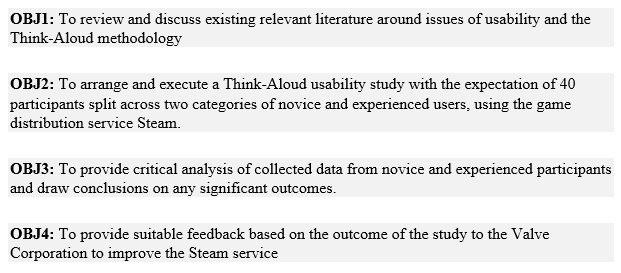
\includegraphics{Screenshots/projectObjectives.png}
\end{figure} 
   
   
   
    
\subsection{Research Questions}
During my project I will attempt too answer the following research questions (RQX). These research questions will be discussed within Chapter 6, Research Discussion. 

\begin{figure}[H]
    \centering
    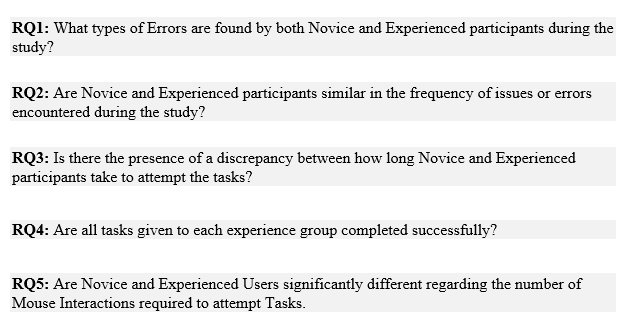
\includegraphics{Screenshots/rqxUpdated.png}
\end{figure}



\section{Structure of this work}
This work will be split into multiple chapters. This chapter, chapter 1 is an introduction to this work, introducing themes of UX research, usability and my projects overall aims, objectives and research questions. Chapter 2, Literature Review, provides a further look into the existing materials for both \gls{ta} methodology, but also for work relating to previous user knowledge and the influence can have upon TA research. Chapter 3, Research Methodology, is an overview on my my UX research was conducted, including what materials, participant criteria and data that I collected as part of this work. Chapter 4, Participant Demographics, presents all of my data collected on my Novice and Experienced participants, including factors such as generic demographics including age, gender and education, secondly questions relating to participant previous experience with gaming such as how many hours spent playing games by each type of participant. Chapter 5, Research Findings, is the presentation of my data collected from my study, with the following data metrics, issue and error detection, Task Duration, Task Completion and Task Mouse Interactions. Chapter 6 Results Discussion, takes this all data sets collected and evaluates the results in context of the research questions presented in Chapter 1.3. Lastly, Chapter 7 Conclusion, summarises the project and presents its limitations and finally suggests some new aspects for further study and expansion on this work.



\chapter{Literature Review}

\section{Literature Overview}
This chapter will discuss existing literature relating to the \gls{ta} protocol. A discussion of the use of Experience as a metric within the testing of applications, especially in relation to \gls{ta} studies will also be discussed.
\section{The Think-Aloud Methodology}
The Think- Aloud protocol (TA) is a form of usability testing whereby test participants are told to verbally communicate there thoughts during tasks of a usability study, or simply to ``think aloud". This could be during the experiment where test organisers would ask participants to verbalise their thought process during the participants attempt to complete tasks, this is refereed to as ``concurrent usability testing" (CTA). Additionally there is also the notion of ``retrospective think-aloud" (RTA) methods, where test participants complete tasks and then verbalise there thought process after the tasks are complete. The concept of Think-Aloud has been developed by Ericsson and Simon, in which they classify three levels of verbalisation \citep{ericsson1998study}. Levels 1 and 2 are the most useful types of data, according to Ericsson and Simon. Type 3 data makes assumptions on how the user infers a task, which could make collected data unreliable. An example they give is to ask users to select only certain items to a criteria, therefore asking users to filter items, which requires some inference on the users part. However as Boren and Ramey writes, the way in which a speaker relays their interpretation of tasks in also influenced by the accompanying practitioner. For instance if a speaker has the expectation of a response from the listening practitioner, but does not receive a response, it could skew their response in a number of different ways.\citep{boren2000thinking}. Therefore TA practitioners should be careful when providing explanations to study participants, to help minimise these potential effects.

These methods have been analysed by various studies comparing variations of Think-Aloud for there associated strengths and weaknesses. Issues have been highlighted by Ramey et al. One issue could include the potential for distraction as some participants may find it difficult to both verbalise there thought processes when attempting tasks during a CTA study, as participants could be influenced by CTA by taking longer to complete tasks, or being unable to complete tasks overall as they cannot concentrate \citep{ramey2006does}. This view is also shared in a 2013 study, although McDonald's et al findings did not find that to be of determent in all their participants. \citep{mcdonald2013thinking}. However many studies argue that by thinking aloud, knowledge on how participants feel in the task can be easily explained in what they say, and how they say it. As Cooke comments, CTA in combination with eye tracking software produces reliable and useful data in how users interact with websites \citep{cooke2010assessing}, as what people say can be verified by the recorded location of their eyes during a CTA test. In a 1991 study, Think-aloud methods were seen to be useful for UX designers as they detect issues that the designers themselves could not detect \citep{wright1991cost}.This has been seen in more recent studies including Van et al, in which they conclude that retrospective and concurrent usability testing leads to the discovery of similar issues, but in different ways \citep{van2000thinking} and \citep{van2003retrospective}. 


\section{Experience as a Metric in Usability Studies}
There has been other studies conducted on that of the user experience, this is in terms of how valid users of different experience levels can be used, and if these groups should be used to test different tasks. This is on the basis that novices and experienced users have prerequisite requirements such as a lack of knowledge in the tested application (for novices), and a minimum level of knowledge for experts. \citep{popovic2000expert}.In several previous studies, novice and expert users were often given different tasks. Faulkner and Wick state that, in "traditional usability testing" a users experience was used to measure different tasks, novice users were useful in determining a programs learnability and experienced users were used to find the most optimal outcome.\citep{faulkner2005cross} However they argue that by using both novices and experts for the same research tasks could lead to more useful data. They also explicitly refer to the flaws of not using multiple levels of experience in detecting flaws in a program, making reference to the "Therac-25" incidents. Therac-25 was a medical accelerator used for radiation therapy, but was also the cause of several patient deaths due to radiation overdoses. One such reason for these overdoses was due to the speed in which experienced users were able to enter commands for the system to process, however as they were familiar with the process they entered the commands too quickly for the Therac-25 system to assimilate. Faulkner and Wick suggest that by employing both novice and expert users, issues such as this could potentially have been detected, although they do not fully explain why, and more concrete examples were absent from this study.

 Novice and expert users have also been used in tests between two distinct versions of a program. For instance, on study focused on two versions of software of a university database dedicated to art resources. The first version had graphical aids, and the second had no graphics elements. The general results showed that novice users improved their ability to use the tested program with presence of graphical cues, versus that with without \citep{dillon1997empirical}. Expert users involved in the study however showed that there was little difference in how effectively they were able to use the program. Therefore if novices were absent from the test this information would not be present at all. The factor of task completion time has also been studied in experience based experiments, including the Novice Expert Ratio method (NEM) method. This methodology concluded that if there was a significant difference of task completion time between novice and expert users, the service being used has usability issues.\citep{urokohara2000nem} Although this can be the case, the issue of familiarity arises. Should a user who is a novice spend more time with a service or product the number of issues they have with a service would decrease, and therefore this metric alone does not necessarily indicate an issue with the product.


\chapter{Research Methodology}

\section{Overview}
This chapter highlights the employed methods of how research was conducted during this project. This includes an overall description of what has been done, followed by an in depth description of each element employed within the project. The individual elements include my collected metrics, tasks given to study participants, how participants were recruited and how they are categorised into Novice and Experienced categories.

\section{Research Methods and Planning}
\subsection{Experiment Procedures}
To begin this project, participants were asked to complete a short pre-study questionnaire (see Appendix B.3), this was to collected basic details and to categorise participants into Novice and Experienced users of gaming services such as Steam. A series of series of individual study sessions were then conducted, lasting around 20-30 minutes per participant. During each session the necessary materials were given to each participant, this included the reasons for the study, any risks of the study to the participant, what data that was to be collected and how it was collected. This included recording the participants voice and the laptop screen for the duration of the experiment using OBS (Open Broadcast Software \citep{OBS2019}) and a microphone (see Appendix B.2). Any questions were answered before the beginning of each session, if the participant had any queries, clarifying that any questions asked during the experiment would not be answered such as how to infer or even complete the six tasks describes further below. Participants were then asked to begin from Task A and sequentially attempt each of the tasks in turn. Once a task was completed the task completion time, whether the task was completed with the expected outcome, the number of mouse interactions and finally any errors, issues or relevant comments made by each participant were recorded using materials seen in Appendix B as they attempted each Task. Due to the recorded data taken via OBS, it was possible to refer back to video and audio logs to confirm any further issues that may have been missed during each session. Conditions were made to be as similar as possible for each test session using a quiet location as well as limiting a number of distractions as possible, equipment and software was prepared the same way for each participant session. The laptop display was 15.6 inches across and in the same brightness settings, a wireless mouse was also provided to be used in the test sessions instead of the laptops track-pad, to provide better ergonomics for the participants in this test and remove the factor of unforgettable study materials influencing the participants. Initially this study was to have  40 participants in total, split into two even groups. However this study involved total of 32 participants, as the process of organising and conducting each study experiment was more time consuming then first considered. It was also challenging to find an equal split in each groups demographics especially with regards to age, which shall be discussed more  Chapter 6 Research Discussion. 

\subsection{Role of the Observer}
During the experiments the Practitioners involvement was as minimal as possible. This was to reduce the potential influence that could have been had upon both types of  participants, although Novice users would likely have been more influenced due to the unfamiliar nature of the tested program. For instance, any questions that the participants had whilst the sessions were happening were not answered. This was to ensure the participant was not influenced in how to proceed with each task. For instance a question such as ``Is this correct?" or ``Am I doing this right?", could not be answered as if a positive or negative response was given to the participant it would likely have changed their actions based on the response and thus contribute to the collection of altered results \citep{alhadreti2016thinking}. Therefore When asked such questions, neutral responds were given and the task continued onward.

\section{Tasks for Participants}
The Steam client was installed onto the testing laptop which all participants used, alongside the same mouse and microphone. A new Steam account was prepared in the following ways; three games that were available on the service were purchased, two of these games where already installed (Hollow Knight, Sid Meier's Civilization 5), and the third uninstalled, Terraria. This was because Terraria was part of Task B which was to try to install a pre-purchased game within the test accounts library. Below are the six tasks that participants were asked to attempt during the study, further illustrated details can be be seen in Appendix B.6. Additionally in Appendix A I have several screen shots from the Steam Client which provide some context to these tasks. Figures 2, 3 and 4 relate to Task A, figures 5 and 6 for Task B, figures 7,8 and 9 for Task C, figures 10, 11 and 12 for Task D, figures 13 and 14 for Task E and finally figures 15, 16 and 17 for Task F. The purpose of these figures is to give a walk through of what an experienced user would do to complete all Tasks successfully, the images are not exact emulators of the Tasks given to the participants, as games were different, but the process of the Task remained the same.

\begin{figure}[H]
    \centering
    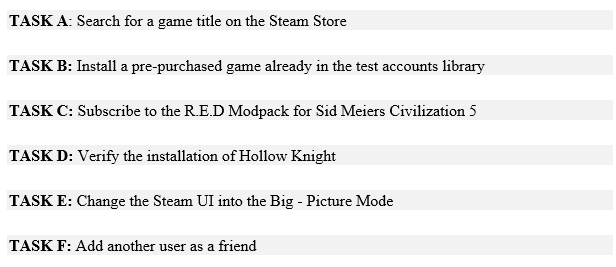
\includegraphics{Screenshots/StudyMaterialScreenshots/tasklist.png}
\end{figure} 

Task A required participants to search the Steam store for a game title, and then subsequently display the store page for the searched game. This task is one of the most common tasks that a Steam user can do, as this is the main service that Valve offers, aside from playing the purchased game which is not a task featured in this study. Additionally the way task is present in a multitude of applications and as such I foresaw that there would not be a huge number of issues or errors from this task, as it is in essence searching a database, which in this case is full of games. 

Task B asked my participants too install a pre-purchased game which is in the test accounts library. This task is relatively common for Steam users, especially if they are installing Steam onto a new PC or laptop, or if they are having issues with a game that requires an re-installation to fix. This task is more complex than task A, but is still relatively straight forward and again I expect fewer issues encountered by both sets of participants, especially those in the experienced category. Experienced participants are likely used to this concept on there respective platforms outside of Steam, such as using a gaming console.  

Task C involved using the Steam Workshop which is an aspect of Steam which community developed modifications available for a large number of titles on the Steam service. This task is the most difficult task of the six. Firstly, many of the participants are unlikely to be familiar with the concepts of modifications in relation to gaming, additionally it is also task that requires multiple interactions on different pages within the Steam client, thus heightening the possibility that participants could become lost within the service. There are also a multitude of different modifications available which could cause some further confusion, especially for Novice participants. However I also expected that Experienced participants would encounter difficulties, as many gaming users do not have an interest in modifying there purchases, and just wish to enjoy the product they purchased as the developers intended.

Task D is another somewhat difficult task. The process of verification involves taking an already installed game and checking that all files that are expected are present within the installation directory. This can be useful for Steam users as many games are hundreds of gigabytes in size and therefore re-installing all of the game data can be extremely time consuming, especially if the user does not have a strong internet connection. Therefore by using verification this can be avoided. However in order to achieve this, a user must find the corresponding properties menu for the game in question, which involves a right-click on the particular game. However this is not sign-posted as can be easily missed, which I again expected many participants of both types to encounter.  

Task E involved changing the \gls{ui} of the Steam Client so that it become more convenient for users who prefer a more console like experience, known as \gls{bpm}. This refers to using a Xbox Controller in order to play games as one example, and therefore forgoing the use of keyboard and mouse as an input method. The \gls{ui} is changed so that visual elements are far larger and can be seen a a greater distance, suitable for use on a large television. Changing to this mode is not extremely difficult and can be achieved in one button press, however due to the unfamiliar terminology I expected some participants to encounter problems in activating it. 

Task F shared similarities to social media such as Twitter or Facebook, as Steam offers the ability to fellow users as friends who can then be played with in game, or general chatting outside of games. Therefore this is quite a simple task and I expected few issues to be encountered when attempting the task regardless of whether the participant was a Novice or Experienced. 

 Efforts were made to make each task independent of one another, so that all tasks could have been attempted regardless if participants completed the previous task or not. When formulating this research, I initially wanted to have users search for a game title as Task A, which then would be followed by them attempting to install that searched game and add thereby add it to the accounts library, by using a free-to-play (F2P) game. However if a participant was unable to complete Task A, they would subsequently fail Task B. Therefore participants were still asked to complete Task A, but Task B was related to a pre-existing game in the Steam library instead, thus eliminating this potential setback, and limiting the collection of Task metrics. 

\section{Study Participants}
As described within the Introduction, the independent variable in this project was the relative skill levels of participants in relation to using gaming services such as Steam. Therefore, what exactly makes a novice user different from that of an experienced user, in the context of \gls{hci} and \gls{ux} UX studies? Novice users have the following characteristics, a limited understanding or no understanding of the tested service or other similar gaming services. This is often someone who is a first time user. Experienced users on the other hand will at least a moderate to high level of understanding and will be familiar with similar services to the tested service of Steam. Participants were spilt into Novice and Experienced groups based on information collected in the pre-study questionnaire (see Appendix B.3), especially regarding later questions including time spent on average using or playing games services and what type of gaming products are owned. There is some variation in this of course, with a wide range of experienced users of different services including PC and other alternatives, however all experienced participants have at least 1-5 hours or more a week played on average, with some exceeding 25 hours on average. 

\section{Data Collection - Prior to the Experiment}
The following subsections discuss how data was collected before the study and what its purpose within the study was. 

\subsection{Observed Behaviours}
As highlighted above, records were made for each of the participants during their use of the Steam service. This was to see what every participant said for each Task and therefore can be directly compared with what what actions they had taken whilst using the service, these actions are often referred to as user journey maps. Aside from what is actually said, the practitioner also checked to see other non-verbal actions that could have been present during each of the sessions, such as participants not being focused on the task, perhaps due to boredom, fear of embarrassment or because they were unsure on how to complete the task.

\subsection{Questionnaires}
Participants were asked to complete a small questionnaire before the experiment took place. The main purpose of this was to categorise participants into the relevant categories of novice and experienced. Basic questions were asked such as name, age and some form of contact. None of this identifying data is published within this project, as to conform with the \gls{uea} privacy policy and \gls{gdpr} law. Information regarding a for of contact such as a mobile phone number was collected should the need have arisen to contact any of the participants, or if they needed to contact me regarding their involvemet. Thus then being able to deal with their data directly, should they request to pull out of the project after their test session.   


\section{Quantitative Data during the Experiment}
The next subsections discuss the quantitative data that I collected during this project, and each data sets purpose.
\subsection{Tools Used During Quantitative Data Collection}
Firstly, hand tools were required in order to collect the various metrics from tested participants. This included data recording sheets in order to take each Tasks Duration, Task Completion and Task Mouse Interactions. Space was present next to each task to record any notable actions or issues encountered by each of the participants, which were also recorded with the microphone, this can been seen in Appendix B.8 and B.9. To collect Task Duration a stopwatch was needed to time each task. The duration of each task was checked via the OBS recording that made for each participant session to confirm the time accurately. Task Mouse Interactions were collected using a program called WhatPulse, which allows the user to track mouse clicks made on a per program basis. 

\subsection{Task Duration}
Aside from error detection, this research also also wished to detect any discrepancies between the Novice and Experienced participants with regard to how long they take to complete each task, if the task was completed (RQX 4). A series of Kruskal-Wallis tests were conducted to determine any significance between the Novice and Experienced categories, using SPSS (Statistical Package for the Social Sciences \citep{SPSS2019}). If a significant difference was present between each group, they it could be indicative that there are usability issues present within the Steam service. However there other metrics must also be collected to provide a more concrete conclusion on the both the usability of the Steam service, and the influence of user knowledge on the \gls{ta} methodology. This metric was taken to answer Research Question Three

\subsection{Task Completion} 
This metric assesses whether the participants were able to complete the task successfully, specifically with the expected outcome. For instance, Task C was to subscribe to the correct modification for Sid Meier's Civilization 5. If the task was not completed or completed incorrectly, it again would be indicative of usability issues during the usage of the Steam service. Much like Task Duration, a Kruskal-Wallis examination of the data between Novice and Experienced participants was conducted using SPSS. Therefore this in combination with Task Duration and Mouse Clicks would help to assess both Novice and Experienced participants as well as the secondary objective of analysing the usability of the Steam client, as well as answering Research Question Four, which asks if all tasks are completed by each set of participants. 

\subsection{Task Mouse Interactions}
Mouse Interactions are how many mouse clicks it takes the participant to complete a certain task, if the task is completed at all. This is tracked by the program WhatPulse. After the participant had attempted each Task, the number of mouse clicks it took them to complete or attempt the task would be recorded. The counter to track the number of mouse interactions would be reset before each Task. With this data collected another set of Kruskal-Wallis examinations were conducted in order to determine any significant differences between novice and experienced participants in the number of mouse interactions taken in order to complete (or attempt to complete) a task, and was also taken to assess and answer Research Question Five. 

\section{Error and Issue Detection}
Recording the number and types of errors encountered by my participants was critical in answering the impact that previous user knowledge has upon the process of concurrent Think-aloud usability testing as well as Research Question One and Two. Therefore as part of this research all issues and errors encountered by both types of participants were recorded on a task by task basis as well as issues encountered in multiple tasks. I have also recorded any general comments made by participants which did not relate to any one particular task. 

\chapter{Participant Demographics}
\section{Overview}
This chapter provides all the data collected on my participants before any experiment was carried out. The purpose of this was to categorise participants into the Novice and Experienced groups. Data collected included generic demographics such as gender, age and highest level of education. More specific data surrounding the participants knowledge on gaming themes such there overall familiarity with games, how long they would play games for per week and what types of outlets they would use in order to play these games was also collected. 

\section{Pre-Experiment Questionnaire - General Demographics}
\subsection{Gender Demographics}
\begin{figure}[H]
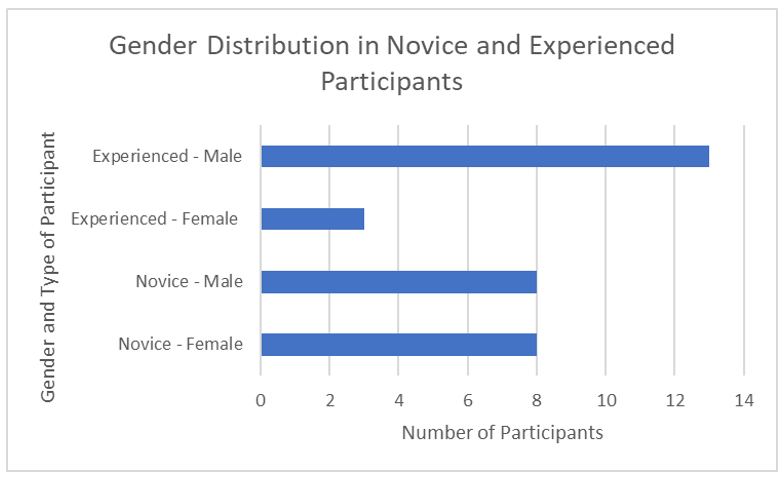
\includegraphics[width=\linewidth]{Screenshots/DemographicsQuestionaires/genderDistribution.png}
\label{GenderDistribution}
\caption{Gender Distribution of Novice and Experienced Participants}
\end{figure}

This graph displays the numbers of female and male participants in both Novice and Experienced categories. On first glance the Novice group is balanced with eight males and eight female participants thus having a 50/50\% split. However male and female participants within the Experienced category are unbalanced with 13 male (81.25\%) to only three female (18.75\%) participants and as such can be considered one limitation in this study, to be discussed later in Chapter 8, Conclusion.  


\subsection{Novice Demographics}
\begin{figure}[H]
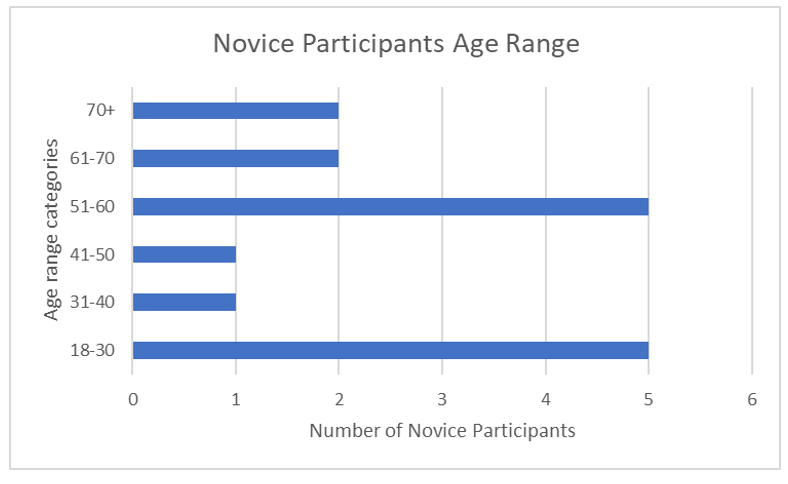
\includegraphics[width=\linewidth]{Screenshots/DemographicsQuestionaires/noviceAgeRange.png}
\label{NoviceAges}
\caption{Novice Age Range}
\end{figure}

This graph shows the distribution of age groups within the Novice category. The two largest groups were participants aged between 18-30 and and 51-60, with each category holding five participants or 31.25\% of the total group population. 61-70 and 70+ categories held two participants each, accounting for 12.5\% of the population each. Lastly 31-40 and 41-50 categories held one participant each thus accounting for 6.25\% for each category in the total sample of participants totalling 16 overall. 

\begin{figure}[H]
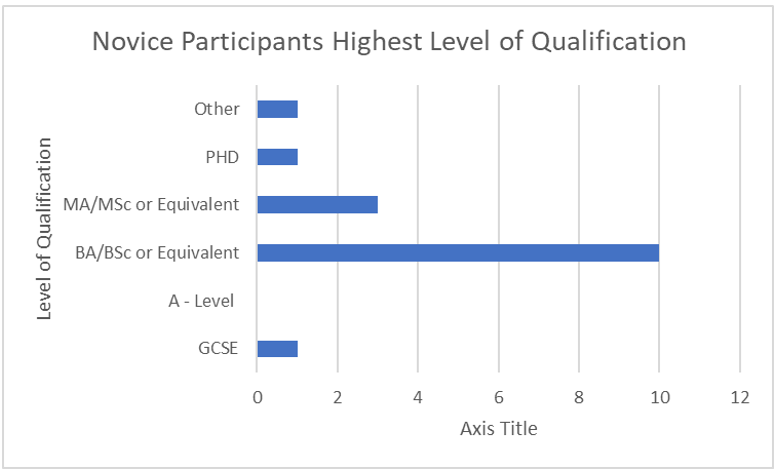
\includegraphics[width=\linewidth]{Screenshots/DemographicsQuestionaires/noviceEducation.png}
\label{NoviceQualifications}
\caption{Novice Participants Highest Level of Qualification}
\end{figure}

There are several levels of qualification that were answered by the novice participants. 10 (62.5\%) of participants holding a BA/BSc or equivalent qualification. Three participants (18.75\%) held an MA/MSc or equivalent. The remaining groups held one participant each (6.25\%) with the exception of the A-Level category with no participants answering that as their highest level of qualification.

\subsection{Experienced Demographics}
\begin{figure}[H]
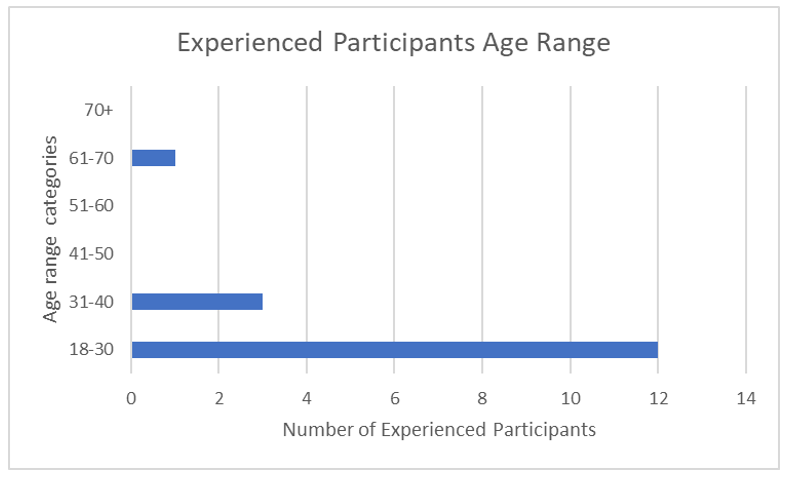
\includegraphics[width=\linewidth]{Screenshots/DemographicsQuestionaires/experiencedAgeRange.png}
\label{ExperiencedAges}
\caption{Experienced Participants Age Range}
\end{figure}

The age range of participants within the experienced category shares a similar issue to that of gender distribution within this category. This is because 12 of the 16 participants were aged in the 18-30 age range thus accounting for 75\% of the experienced population sample. Therefore only three participants were aged between 31-40 and only one participant aged in 61-70 category. However this distribution is in keeping with general trends within the gaming industry with those aged between 18-30 being one of the most popular users of games services, extending up to the age of 40 according to 2017 global statistics \citep{gamersChristinaGough2017}. 

\begin{figure}[H]
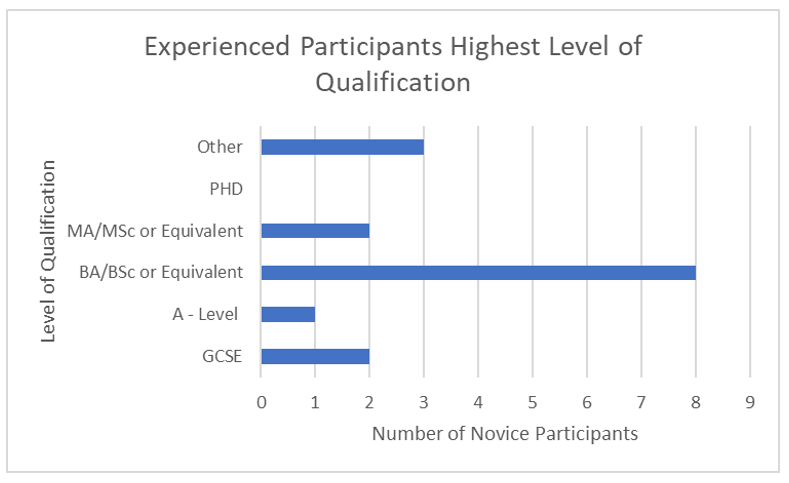
\includegraphics[width=\linewidth]{Screenshots/DemographicsQuestionaires/experiencedEducation.png}
\label{ExperiencedQualifications}
\caption{Experienced Participants Highest Level of Qualification}
\end{figure}

Similarly to that of the Novice participants, there was a wide range of levels of education, with the same majority of participants holding at least a BA/BSc or equivalent qualification. However those who held a BA/BSc or equivalent qualification only totalled eight or 50\% of the sample population, as compared with 12 or 75\% of the Novice sample population. Three (18.75\%) participants held qualifications that did not fit into other categories, two holding (12.5\%) MA/MSc or equivalent, a further two (12.5\%) with at least GCSE and one participant with A-level qualifications. 

\section{Novice Pre-Experiment Questionnaire Gaming Queries}
The following section details some key information that I asked my Novice participants before and after there involvement in my study, with specific queries relating to their knowledge on gaming services and their thoughts on the \gls{ta} process during there testing session.

\subsection{Gaming Familiarity}
\begin{figure}[H]
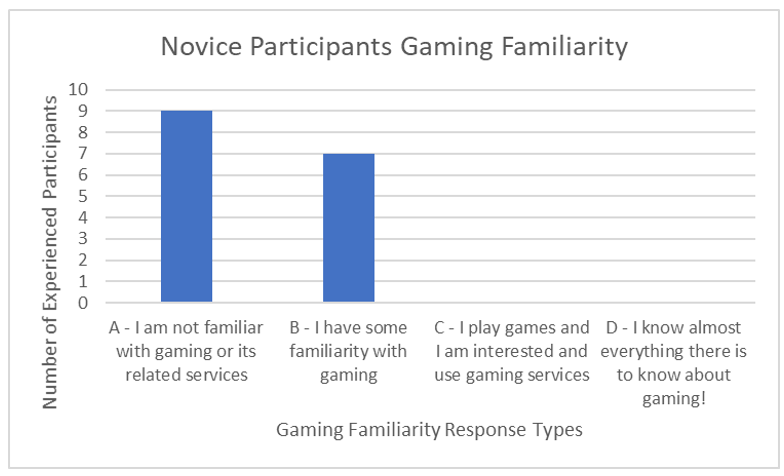
\includegraphics[width=\linewidth]{Screenshots/DemographicsQuestionaires/noviceQuestionaireData/noviceParticipantsGamingFamiliarity.png}
\label{NoviceGamingFamiliarity}
\caption{Novice Participant's Familiarity with Gaming}
\end{figure}

This graph details how my Novice participants responded to the question asking them how familiar they were with gaming concepts. This could be personally through their own usage, or vicariously such as with a sibling or child's interest in gaming. Unsurprisingly all my novices responded with A or B which means that their overall knowledge in gaming is limited, as anticipated when formulating this research. Out of 16 participants, nine or 56.25\% responding that they were not familiar with gaming at all, with the remaining seven or 43.75\% of participants answering B, thus holding some limited knowledge within gaming. 

\subsection{Gaming Devices Ownership}
\begin{figure}[H]
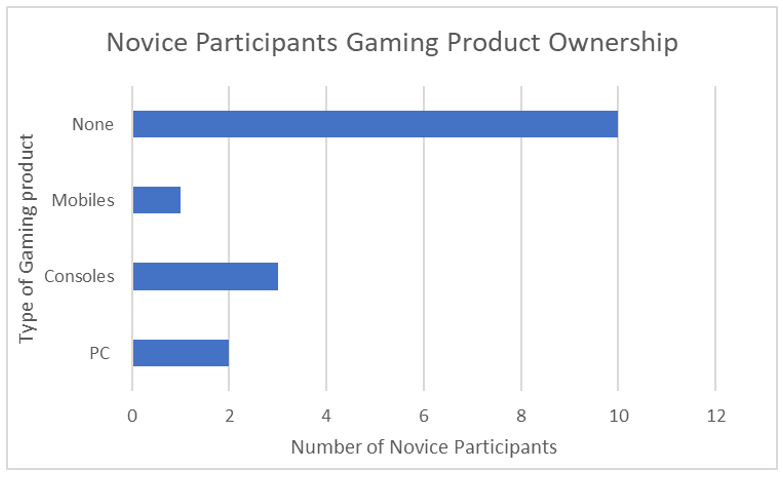
\includegraphics[width=\linewidth]{Screenshots/DemographicsQuestionaires/noviceQuestionaireData/noviceGamingOwnership.png}
\label{NoviceGamingOwnership}
\caption{Novice Gaming Product Ownership and Usage}
\end{figure}

After asking the Novice participants for their overall gaming knowledge, a question regarding which devices they owned and used was also asked. The majority of the 16 participants answered that they owned no dedicated gaming devices and devices capable being used for gaming were not used for that purpose, totalling ten participants. There were six participants who were in the sample minority. Three participants (18.75\%) answered that they owned Consoles such as a Sony PlayStation 4, two participants (12.5\%) owning a PC used for gaming purposes, and one novice participant (6.25\%) who used their mobile phone to casual play games on. 

\subsection{Time Spent Gaming}
\begin{figure}[H]
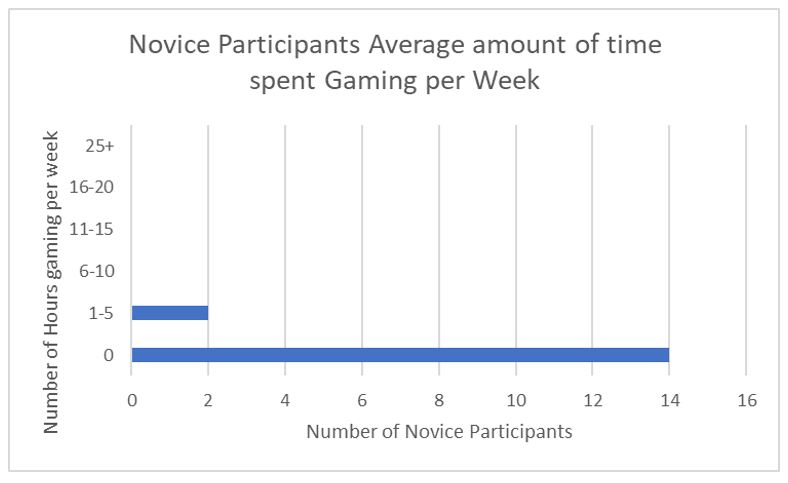
\includegraphics[width=\linewidth]{Screenshots/DemographicsQuestionaires/noviceQuestionaireData/noviceTimeSpentGaming.png}
\label{NoviceTimeGaming}
\caption{Novice Participants average Time Spent Gaming per week}
\end{figure}

This data is a further expansion to the data collected in Figure 4.7. As expected the majority of participants answered that they did not spend any time per week gaming on any devices. Only two participants (12.5\%) answered that they played for a brief time period of 1-5 hours a week. Thus confirming that my participants were complete novices to gaming, or at most extremely casual players of games. 

\section{Experienced Pre-Experiment Questionnaire Gaming Queries}
The following section details some key information that experienced participants were asked, before and after their involvement in my study with specific queries relating to their knowledge on gaming services and their thoughts on the \gls{ta} process during there testing session.

\subsection{Gaming Familiarity}
\begin{figure}[H]
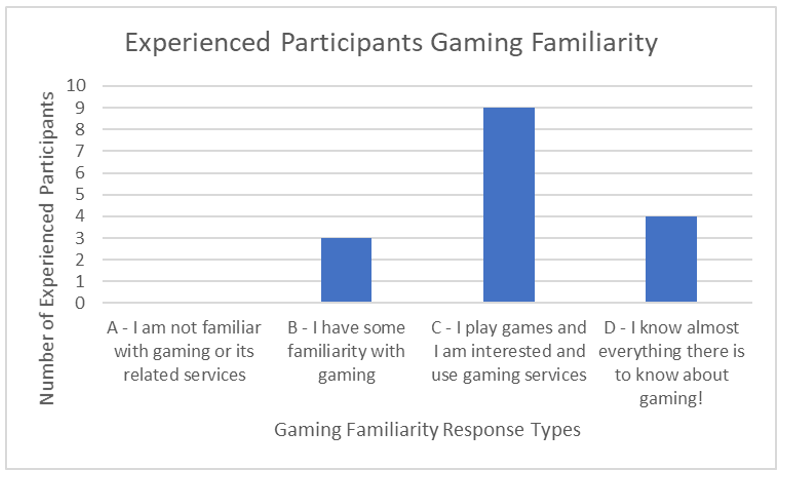
\includegraphics[width=\linewidth]{Screenshots/DemographicsQuestionaires/experiencedQuestionaireData/experiencedParticipantsGamingFamiliarity.png}
\label{ExperiencedGamingFamiliarity}
\caption{Experienced Participants Familiarity with Gaming}
\end{figure}

This figure shows the response from my experienced participants in relation to gaming familiarity. Nine participants (56.25\%) responded with option C, 4 (25\%) with option D, and three (18.75\%) with option B. No participants in the experienced category answered with response A, which was expected as if they had, they would have placed them into the Novice category.

\subsection{Gaming Devices Ownership}
\begin{figure}[H]
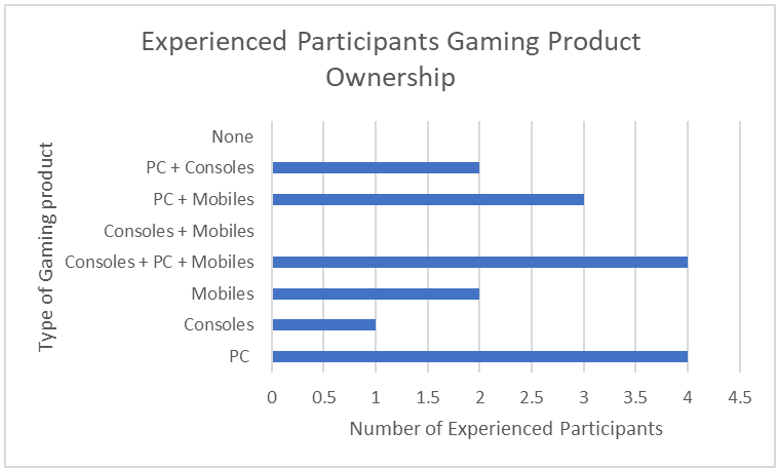
\includegraphics[width=\linewidth]{Screenshots/DemographicsQuestionaires/experiencedQuestionaireData/experiencedGamingOwnership.png}
\label{ExperiencedGamingOwnership}
\caption{Experienced Participants Gaming Product Ownership and Usage}
\end{figure}

This figure is more diverse then that of the Novice counterpart (see Figure \ref{NoviceGamingOwnership}). Experienced participant's gave a series of answers including that of hybrid answers which included two or more options for which outlets they use for gaming. The most common outlets were PC and PC,Console and Mobile use, with four participants in each category accounting for 50\% of the sample population together. Three participants (18.75\%) answered that they used PC and Mobiles, two answered that they owned only mobiles and another two answered that they owned a PC and a gaming console accounting for a further 25\% of the sample population. Only one participant answered that they only owned a gaming console. Interestingly no participants answered that they owned consoles and mobiles together for gaming purposes. Therefore this sample has a wide range of participants with different gaming devices, and therefore expectations on how they would work, especially regarding UI/UX elements.

\subsection{Time Spent Gaming}
\begin{figure}[H]
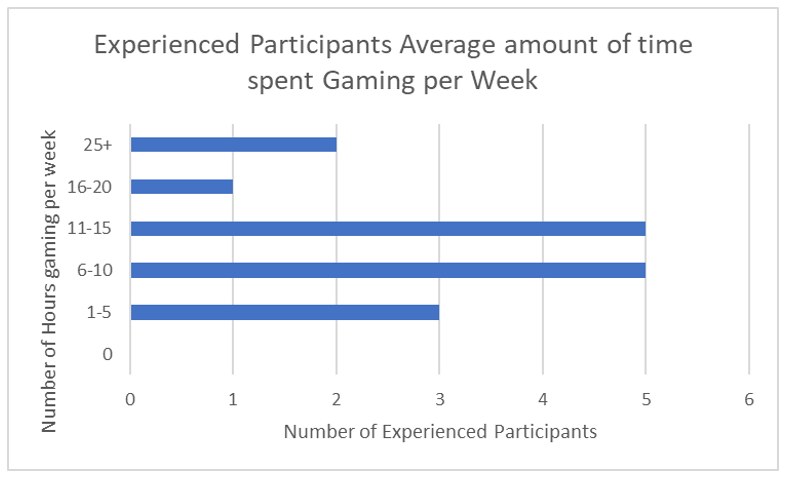
\includegraphics[width=\linewidth]{Screenshots/DemographicsQuestionaires/experiencedQuestionaireData/experiencedTimeSpentGaming.png}
\label{ExperiencedGamingTime}
\caption{Experienced Participants average Time Spent Gaming per week}
\end{figure}

This figure shows that the experienced participants have a varied amount of time spent gaming in an average week of there's, with five participants in 6-10 and 11-15 hours each, thus accounting for 62.5\% of the population. Three participants answered that they played between 1-5 hours a week, which two of the novice participants also answered. However due to other factors such as gaming familiarity and device ownership, these participants are still categorised as experienced participants, despite the similarities to those Novice participants who answered the same way with this metric. Two participants answered that they played over 25 hours a week and as such are considered the most experienced participants. One participant answered that they played 16-20 hours a week and thus they were another highly experienced gaming user. Overall, my experienced category was quite diverse regarding this specific metric.


\section{Post Experiment Questionnaire}
\subsection{Novice Participant Responses}
\begin{figure}[H]
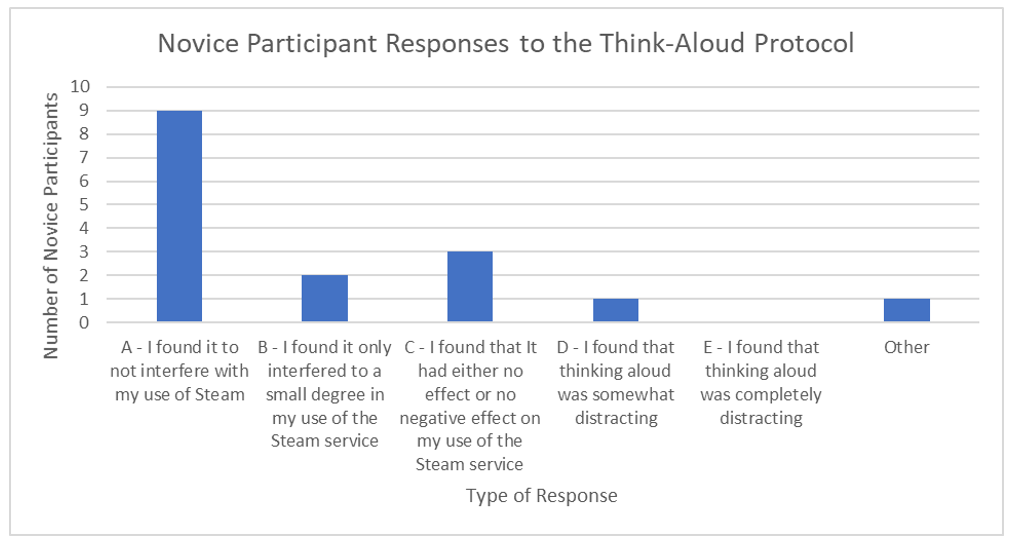
\includegraphics[width=\linewidth]{Screenshots/DemographicsQuestionaires/noviceQuestionaireData/noviceTAP.png}
\label{NoviceTAP}
\caption{Novice Participants responses to the Think-Aloud Protocol}
\end{figure}

This graph shows the distribution of answers given by Novice participants following the experiment regarding the \gls{ta} Protocol. Participants were asked to rate there thoughts on the \gls{ta} methodology, in terms of how they thought it effected there ability to complete the test. For instance, did Thinking aloud distract Novices in there attempts at using the program? This graph shows that not to be the case for the majority of participants. Nine participants (56.25\%) answered that with response A and thought that Thinking allowed did not distract them whilst using the Steam service. A further two did respond that Thinking aloud did interfere with there use of Steam to a minor degree. However one participant found that concurrently Thinking aloud was of somewhat detrimental to the testing process, elaborating that they could not really talk and use the program at the same time. Three participants found the \gls{ta} Protocol has no effect on there use of Steam. Interestingly the last participant found that by thinking aloud it actually helped them use the Steam program, this is indicated by the ``Other" response. 

\begin{figure}[H]
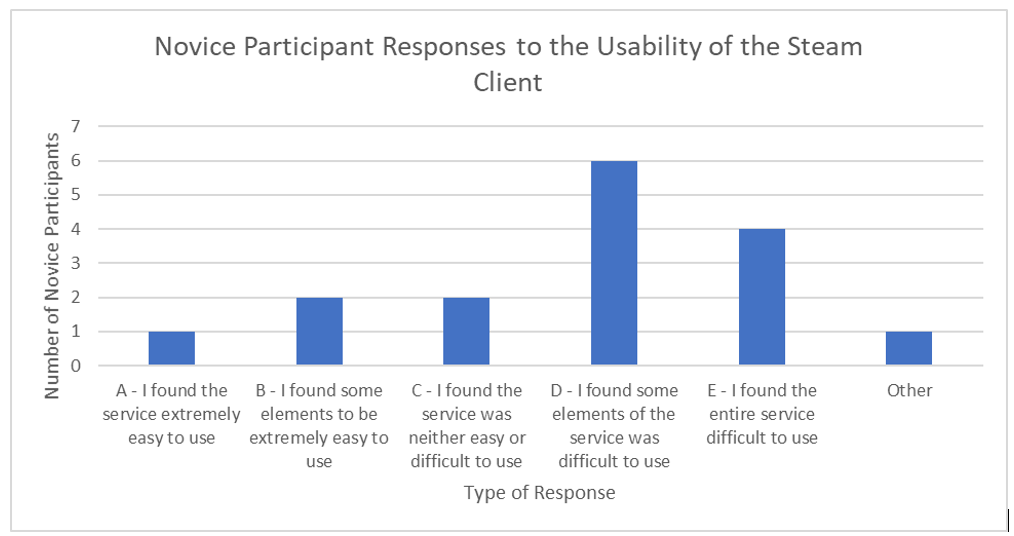
\includegraphics[width=\linewidth]{Screenshots/DemographicsQuestionaires/noviceQuestionaireData/noviceSteamClient.png}
\label{NoviceSteamUsability}
\caption{Novice Participants responses to the Usability of the Steam Service}
\end{figure}

When asked what there thoughts were on the Steam interface most Novice participants responded that they found some of the service difficult to use. This response was given by six participants with a further four saying that the entirety of Steam was difficult to use. A further participant gave the response ``D/E" as indicated by the ``Other" category. This is somewhat perplexing, but still the participant gave Steam a negative usability rating. Thus, category D, E and the hybridised answer accounted for 11 participants or 68.75\% of the sample population. Conversely two novices found that some elements were extremely easy to use, with only one novice saying that they found the entire service easy to use, therefore making up 18.75\% of the total novice sample. The last two participants gave a neutral rating to the usability of Steam regarding the six tasks they had attempted and made up the final 12.5\% of the novice sample population.

\subsection{Experienced Participant Responses}
\begin{figure}[H]
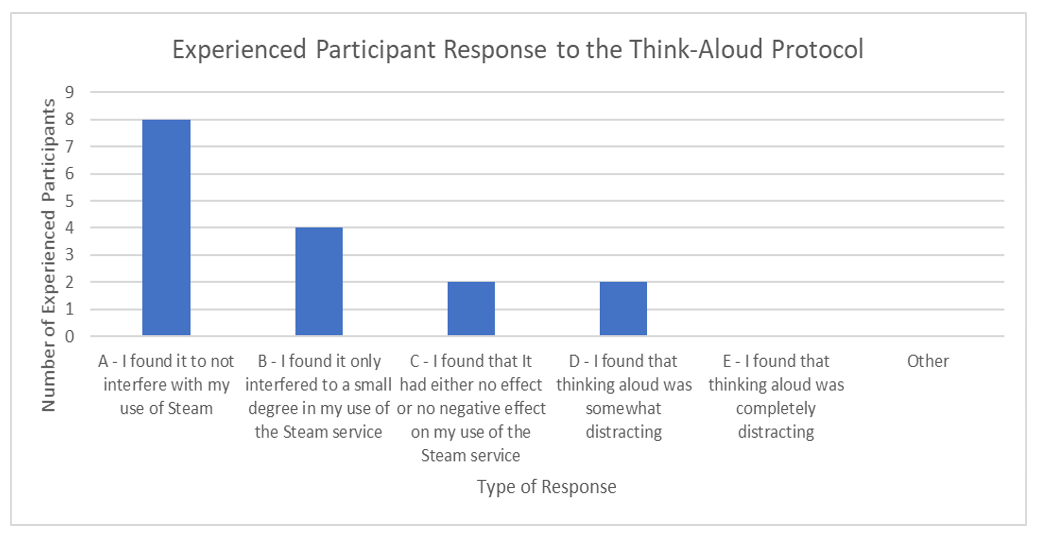
\includegraphics[width=\linewidth]{Screenshots/DemographicsQuestionaires/experiencedQuestionaireData/experiencedTAP.png}
\label{ExperiencedTAP}
\caption{Experienced Participants responses to the Think-Aloud Protocol}
\end{figure}

When asked for their thoughts on the \gls{ta} methodology, most experienced participants reacted similarly to that of Novices, with the majority finding that concurrently thinking aloud did not impact their usage of the Steam service. Eight participants answered that Thinking aloud to not interfere with Steam, with a further four saying that it only interfered there use of the program to a small degree, thus account for 75\% of participants. Only two participants (12.5\%) answered that Thinking-aloud was distracting during the experiment. The remaining two participants (12.5\%) answered that Thinking aloud did not impact them in any way at all. 

\begin{figure}[H]
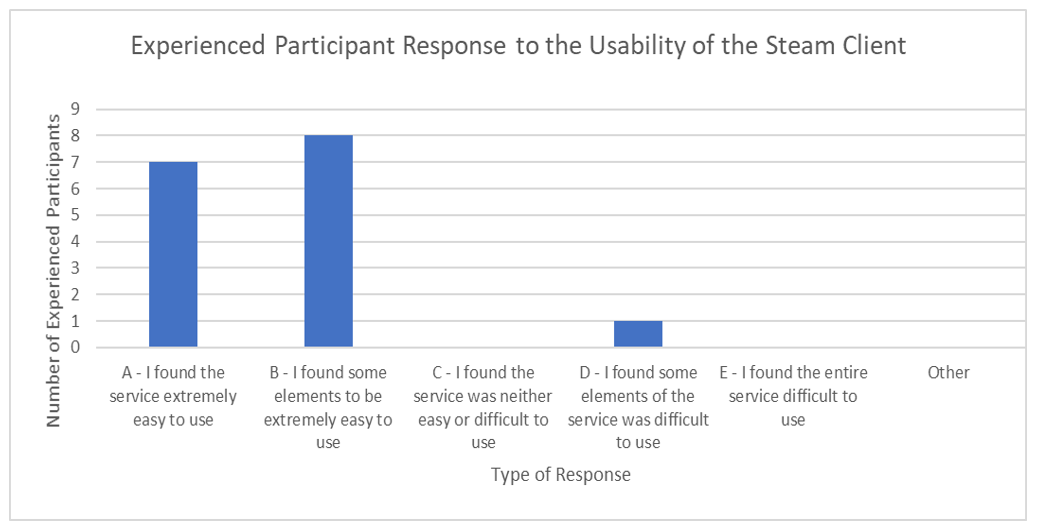
\includegraphics[width=\linewidth]{Screenshots/DemographicsQuestionaires/experiencedQuestionaireData/experiencedSteamClient.png}
\label{ExperiencedSteamUsability}
\caption{Experienced Participants responses to the Usability of the Steam Service}
\end{figure}

Lastly, as expected the majority of the experienced participants responded positively when asked about the usability of the Steam service. Only 1 participant answered that they found the service to be somewhat difficult to use, especially with regards to Task C and D. The remaining 15 participants however reacted positively, with 7 participants saying that the service was extremely easy to use, and the remaining 8 saying that some elements were extremely easy. Thus saying that for the most part Steam seemed to be quite an innovative service.


\chapter{Research Results}
\section{Overview} 
This chapter has my analysis of my participants usage of the Steam service during the Concurrent Think-Aloud study. This analysis includes the following data metrics; Errors and issues encountered, Task Duration, Task Completion and Task Mouse Interactions, spilt between the Novice and Experienced groups. Kruskal-Wallis tests were used to assess the difference between Novice and Experienced participants with the four metrics. These Kruskal-Wallis tests have been calculated at the 95\% confidence interval, therefore results that equal 0.05 or less mean that there is a significant difference and the null hypothesis is rejected that there is no difference.  


\section{Error and Issue Detection}
The following section details all notable errors and issues that were encountered by both sets of participants during this UX study. This is followed by the most common issues that were encountered by both experience groups. Issues refer to a problem caused by the user directly, whereas errors are were the service behaves unexpectedly. An example of an issue, is navigating to the wrong part of the service when attempting a task, such as clicking upon the wrong Workshop for Task C. An example of an error could be something like a black screen, or a \gls{ui} such as flickering or images and text not being scaled correctly. Issues were the most common type of problem encountered, and very few errors were experienced by either novices or experienced participants. Therefore as such Steam is a well built system, but it does have some frustrating elements which newer users will encounter and could be described as somewhat convoluted. Additionally I have also conducted a Kruskal-Wallis test to determine any significance difference between Novice and Experienced participants regarding the number of issues and errors encountered during their usage of the Steam service. This has been conducted with each task, issues in multiple tasks,generic issues and all issues per participant.

\subsection{Novice Participant Error and Issues}
\begin{table}[H]
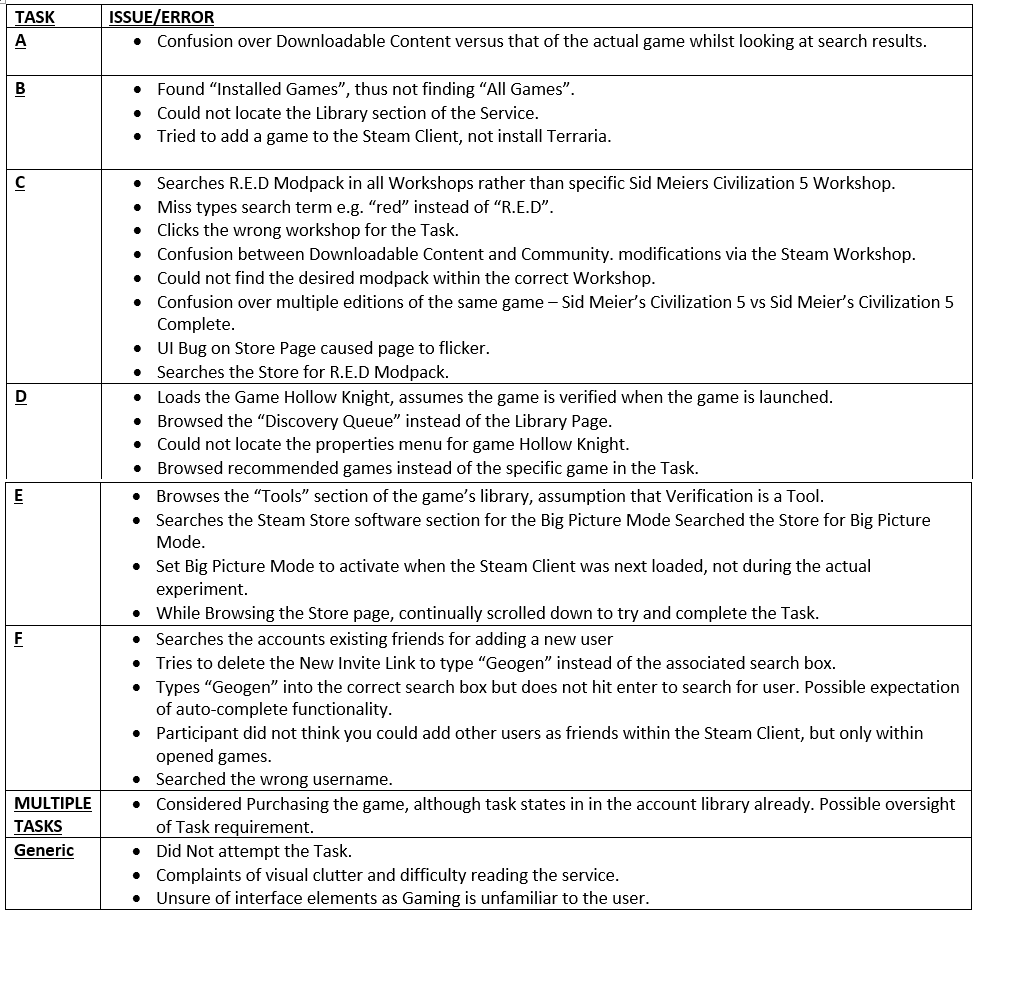
\includegraphics[width=\linewidth]{Screenshots/ErrorRecords/Novice/noviceAllErrors.png}
\label{NoviceErrorsList}
\caption{All Novice Issues and Errors Detected}
\end{table}

Table 5.1 shows all issues and errors that were encountered by my Novice participants during there use of the Steam program. In total there were 30 unique issues encountered which has been presented within the table. However there were variations upon these errors but they were too similar to deem them as a separate error and as such are not present within this table. It is clear that Task C proved the most challenging for the Novice sample with a total of eight out of 29 issues, accounting for 27.5\% of all issues. This was somewhat expected as was stated in Chapter 3, Task C was deliberately more complex task, and as there was the expectation of more issues than other tasks.  Surprisingly Task F had several a total of five unique errors despite the relative similarity to other more commonly used services such as social media, as the task was to add another user as a friend, much like on those other platforms.

\begin{figure}[H]
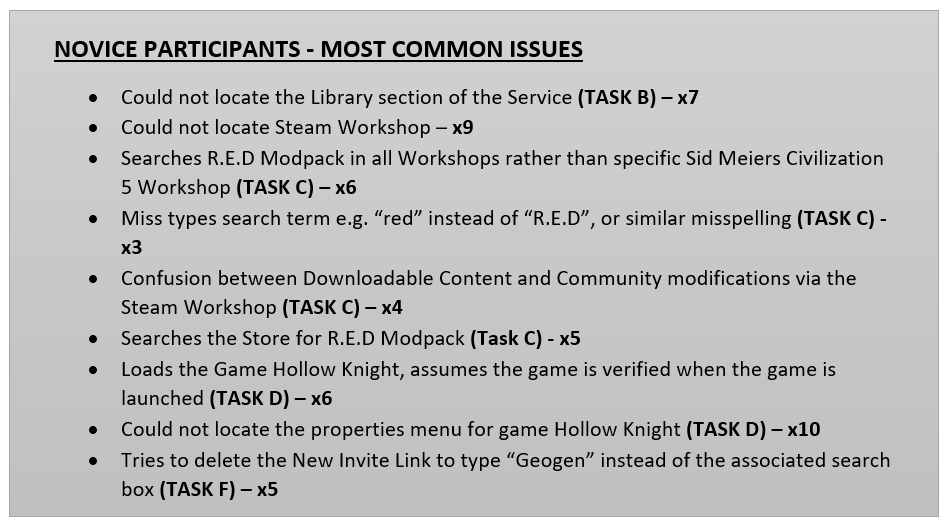
\includegraphics[width=\linewidth]{Screenshots/ErrorRecords/Novice/noviceMostCommonIssues.png}
\label{NoviceMostCommonErrors}
\caption{Most Common Issues encountered by Novice Participants}
\end{figure}

The issues displayed in Figure 5.1 show that the most common issue was in relation to Task D, the verification of a games files and being unable to locate the correct interface element to initiate this process. The prevalence of this issue is not entirely unexpected, as Novice users are less familiar with gaming themes, the word ``verification" is in part the reasoning for why this particular task proved difficult. However this issue has highlighted an issue with the Steam client in how this functionality is shown within the Steam client. A user must know that they have to right click upon the desired game to display the games properties menu, 10 participants failed task D because of this reason as this function is not at all obvious for a new user. Task D is also interesting due to the existence of another issue, that is six novices loaded the game ``Hollow Knight" as they believed that the Task was a trick question and that verification was irrelevant. Therefore the inclusion of this task has highlighted to me that the selection of tasks, and the wording of the task influence generation of issues as well as the service tested itself.

Task C also had three very common issues, which are all directly related to one another as they regard the search functionality of the Steam client. Task C asked users to find a modification for Sid Meier's Civilization 5, which is found within the Steam Workshop functionality. Most users attempted this task in a logical way, by searching for the desired modification, however where the participant searched provided to be problematic for several novice users, by entering ``R.E.D modpack". However several users entered this search term into the search for all game workshops and therefore did not find the desired subscribe tool as the task required. Five other novices decided that they would try to search for the modpack within the steam store page, thus returning products to buy with the word ``red" within them, and therefore irrelevant results for the task. 

Task F's main issue was partially a layout issue as five Novices did not see the search functionality for adding fellow users by name, in the test case ``Geogen". Instead Novices were drawn to using the \gls{nil}. The intended purpose of NIL is to send a link to the desired user by email or SMS, thus requiring an external device in order to connect two users together. Once a link is generated it can only be shared or deleted. Five users however decided to try to type the desired user name of ``Geogen" into the NIL but were unable to do so, and thus became puzzled at the lack of functionality and thus become unable to complete the task correctly.

\subsection{Experienced Participant Error and Issues}

\begin{table}[H]
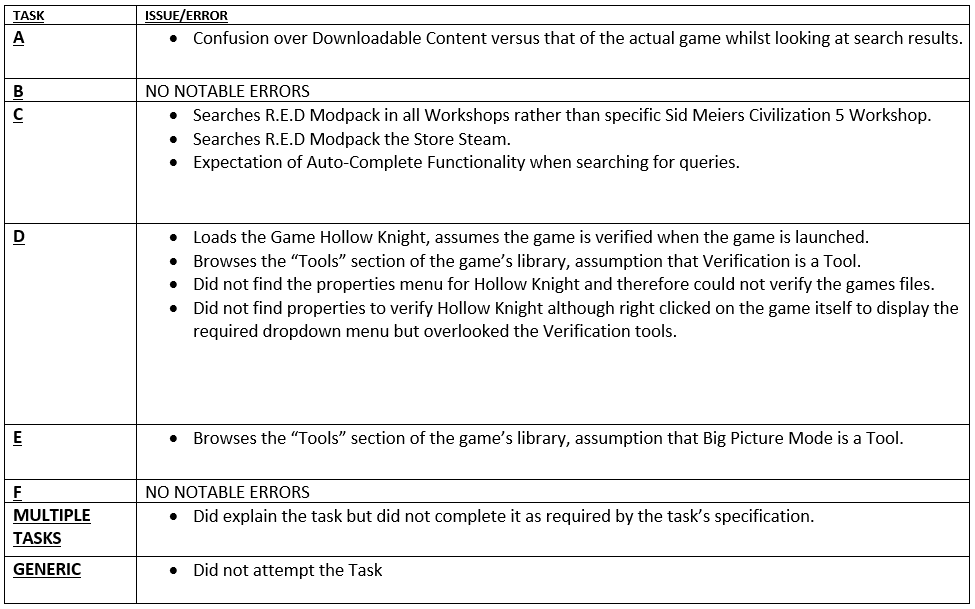
\includegraphics[width=\linewidth]{Screenshots/ErrorRecords/Experienced/experiencedAllErrors.png}
\label{ExperiencedErrorsList}
\caption{All Experienced Issues and Errors Detected}
\end{table}

Table 5.2 is the Experienced total issues and errors encountered during the study. In total there were fewer issues and errors encountered compared to that of the novice participants with a total of 11 overall unique issues. Similarly to that of the Novice participants however, was the presence of issues in Task C , with identical issues being encountered by some of the participants. Another notable aspect is that Task B and task F had no notable issues with the Experienced participants with all participants successfully completing these tasks. Fewer generic issues were also detected by Experienced Participants. 

\begin{figure}[H]
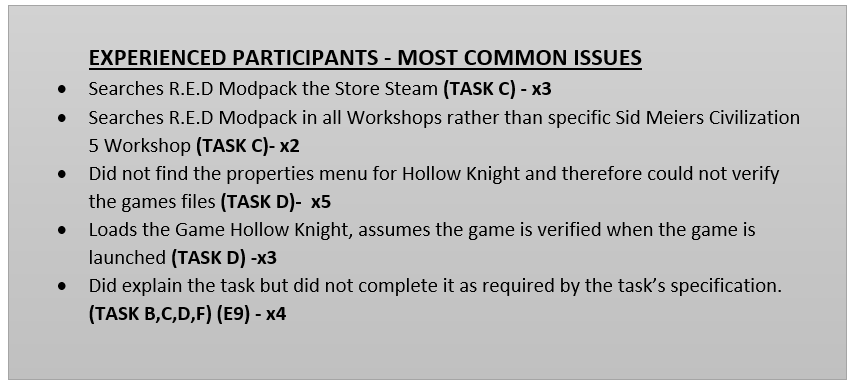
\includegraphics[width=\linewidth]{Screenshots/ErrorRecords/Experienced/experiencedCommonErrors.png}
\label{ExperiencedMostCommonErrors}
\caption{Most Common Issues encountered by Experienced Participants}
\end{figure}

This figure shows the most common issues that were encountered during the Novice testing session. Task D had the most common issue, as five participants out of 16 were unable to locate the properties menu needed to access the verification tools. This issue was very common in the experienced category as well, and therefore shows that Novice and Experienced participants do encounter similar issues during this particular study. Task C also had the same type of issues encountered by Novice participants, whilst trying to find the R.E.D Modpack and using the wrong searching tools. The most notable other type of issue was in the case of one participant (Participant E9) who when asked to complete the tasks they explained how they were going to use the program in order to complete the task, but did not then proceed to complete the tasks in the the manner they described, this behaviour was exhibited during Tasks B,C,D and F but not Task A or E. Although the way in which participant E9 explained their indented use of would have caused them to complete the tasks correctly, they way in which they responded highlights the importance of how the Tasks are explained to the participant, and thus the role of the practitioner cannot be understated during similar Concurrent Think-Aloud studies.

\subsection{Error Type Summary}
It can be summarised that based on this data, the types of errors encountered are broadly similar in both experience categories. There are some exceptions to this, with Experienced participants finding no specific issues with Task B or Task F. However experienced participants did display more issues regarding multiple tasks.

\subsection{Number of Errors By Experience Group}
\begin{table}[H]
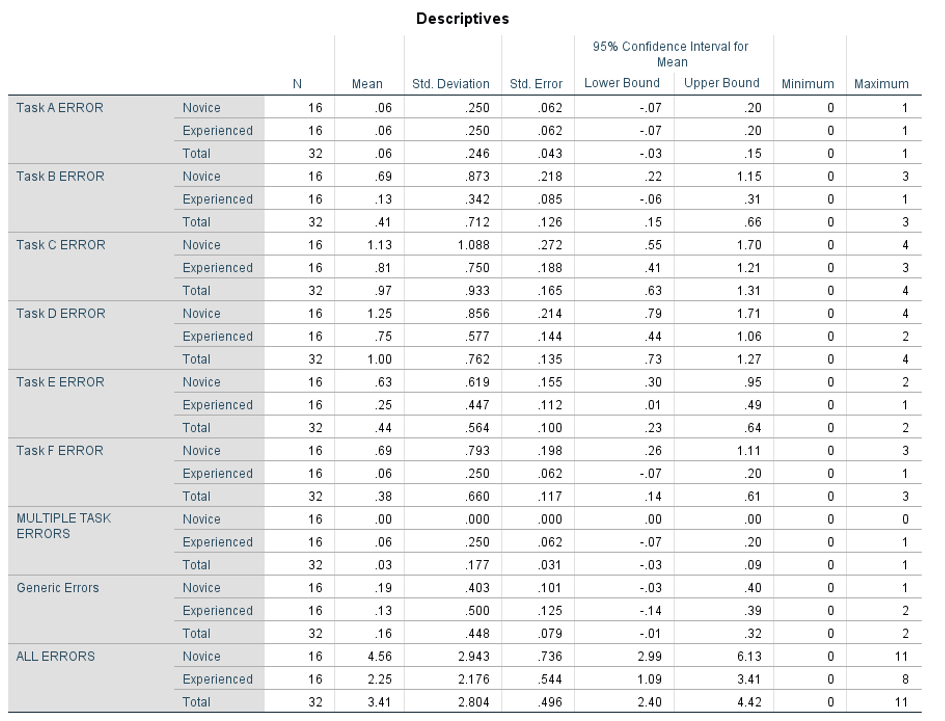
\includegraphics[width=\linewidth]{Screenshots/ErrorRecords/errorBreakdownDescriptives.png}
\label{DescriptivesErrorsPerGroup}
\caption{Descriptive Statistics for Number of Issues Encountered by Experience Group}
\end{table}

Table 5.3 shows descriptive statistics taken from both the Novice and Experienced participant groups regarding the number of errors encountered per group type. All samples were used during this analysis with 16 participants within each group. Task C and D show the highest average mean issues detected within the Novice category, with 1.13 and 1.25 errors detected per participant on average for Task C and D respectively. This trend continues with Experienced Participants with 0.81 and 0.75 issues detected for Task C and D respectively. As anticipated Novices had a higher frequency of errors overall compared to that Experienced Participants, with 4.56 issues discovered by Novices versus that of only 2.25 issues found by Experienced participants on Average, although the highest number of issues detected was 11 for a Novice participant and 8 for an experienced. Attention should be paid to the results regarding the lower bounds of several tasks, as some of these results return negative values, these values should be ignored and considered as zero. This is due to the fact that participants cannot encounter a negative amount of issues during their usage of Steam or other tested services in usability testing.

\begin{table}[H]
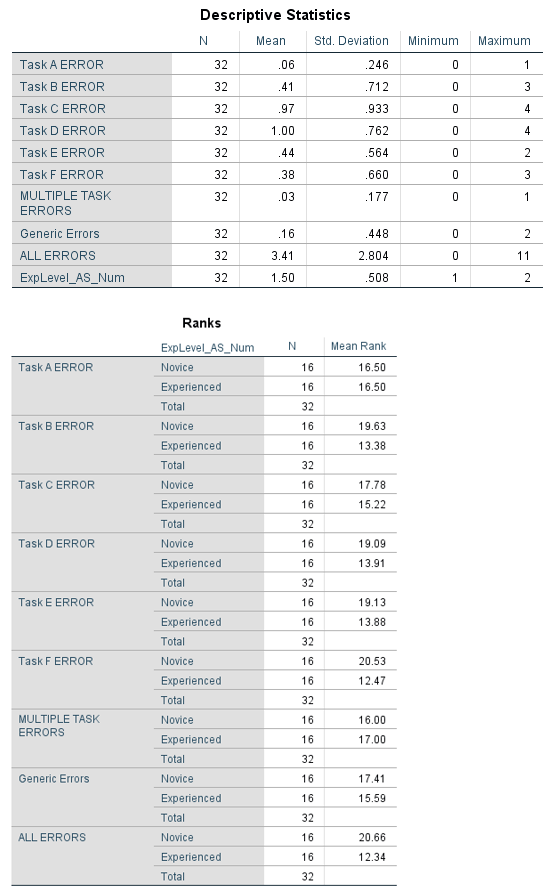
\includegraphics[width=\linewidth]{Screenshots/ErrorRecords/kwDescriptiveErrors.png}
\label{KWErrorsPerGroup}
\caption{Kruskal-Wallis Examination for Number of Issues Encountered by Experience Group}
\end{table}

Table 5.4 shows a condensed version of Table 5.3 with all participant data combined in a Task by Task format, retaining core descriptive statistics. However the second table shows the Mean rank distribution of errors encountered by participants on an experience level basis. As can been seen within this table, the majority of the results show a higher Mean rank for Novice participants in all categories with the exception of  Task A and Multiple Task Errors. Task A shows an equal Mean rank as only one type of error was encountered during this study between the two groups. The Mean rank of multiple task errors can be explained by the results of participant E9 which was explained in Figure 5.2. These results partially answer one of my research questions (RQX2), as it shows that more errors are detected by Novice participants than Experienced ones with regards to the entire sample population of each category.

\begin{figure}[H]
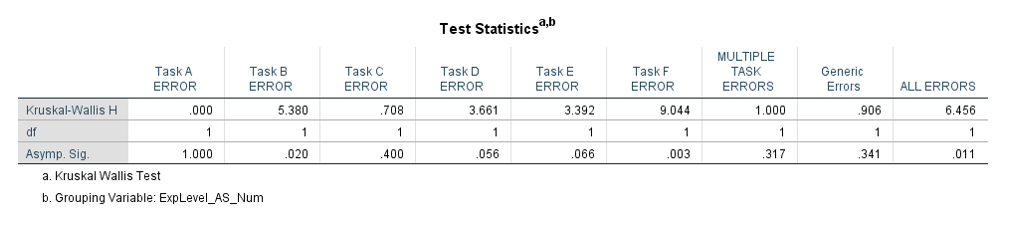
\includegraphics[width=\linewidth,height=6cm]{Screenshots/ErrorRecords/kwErrorsByParticipant.png}
\label{KWErrorsPerGroup}
\caption{Kruskal-Wallis Examination for Number of Issues Encountered by Experience Group}
\end{figure}

Figure 5.3 are the results of a Kruskal-Wallis examination with the numbers of errors detected between Novice and Experienced participants, as calculated at a 95\% interval. On a Task by Task basis, there is no significant difference in Novice and Experienced participants regarding the number of errors detected. This is with the exception of Task F, which shows a Assumption figure of 0.03.  Interestingly, the result for the All errors category also shows that there is no significant difference between the two experience groups, although it is close to the threshold of 0.05 compared with all other Task results. Therefore, it Novice and Experienced participants are not significantly different in regard to the number of individual issues and errors experienced on a per participant basis. However, as shown by the Table 5.4 more errors were detected by the Novice sample population overall compared with the Experienced sample population. 

\section{Task Duration}
The following section details collected data from participants in regards to each tasks duration. Each task's data had a Kruskal-Wallis test performed between Novice and Experienced data sets to ascertain if there was any significant difference between the two groups. Two sets of descriptive data also accompany these results, as to show various variations between the data sets.

\begin{table}[H]
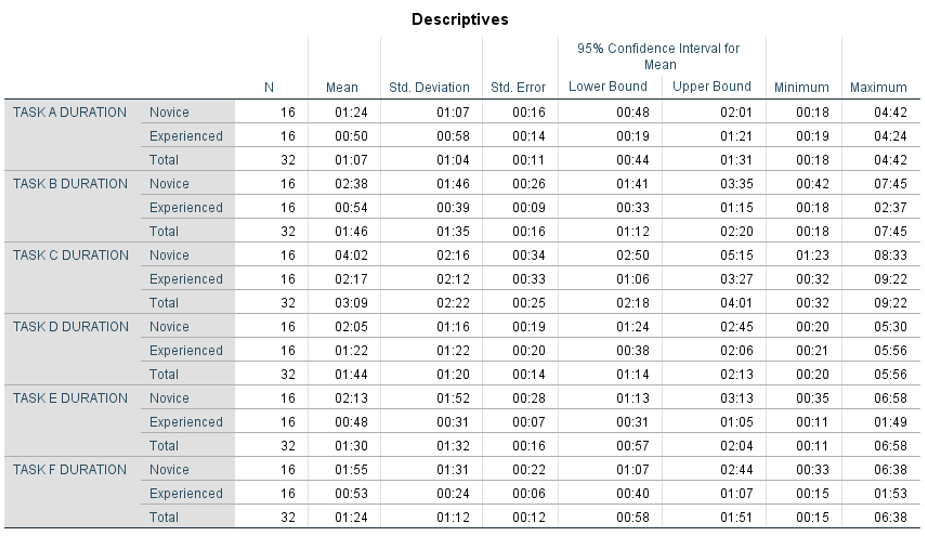
\includegraphics[width=\linewidth]{Screenshots/UXResearchDataFiles/UXTaskDurationData/anovaDescriptivesTaskDuration.png}
\label{DurationOverallStats}
\caption{Task Duration - Descriptive Statistics Novices and Experienced Participants}
\end{table}

This table displays several useful descriptive statistics, including the Mean, Standard Deviation,Standard Error, Minimum value and Maximum values. Critically this data set displays the upper and lower bounds of the data set to a confidence interval of 95\%, for both Novice and Experienced participants and for all tasks attempted. It should also be noted that all tasks data was included, therefore totalling 32 pieces of data per task and 192 pieces of data overall, whilst assessing Task Duration. The longest average time spent on one particular Task for Novice participants was Task C with one participant taking 08:33 minutes to attempt the Task, of further interest is the longest Experienced participant time for one task, which was also Task C taking 09:22 minutes to complete which is surprising. However the majority of these statistics describe a trend that I had expected, that Novice participants took longer to attempt the same tasks as Experienced participants. Task C still proved to be the longest Task on average for both Novice and Experienced participants, which I anticipated as Task C was the most difficult task to complete.  

\begin{table}[H]
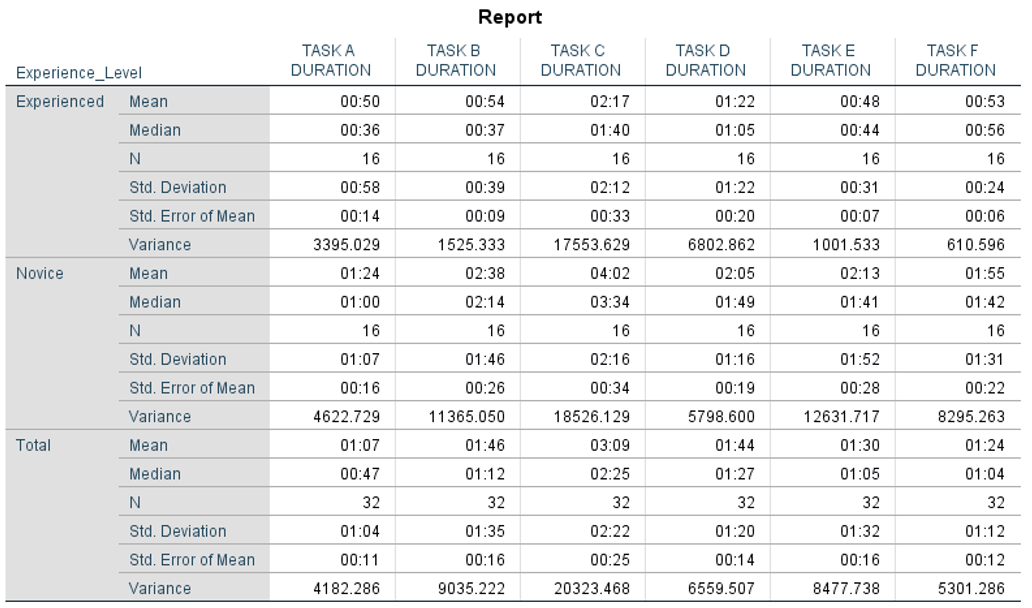
\includegraphics[width=\linewidth]{Screenshots/UXResearchDataFiles/UXTaskDurationData/taskDurationOverallEdited.png}
\label{DurationOverallFurtherStats}
\caption{Task Duration - Further Descriptive Statistics Novices and Experienced Participants}
\end{table}

Further to Table 5.5 this descriptive table shows the variance in the data sets. It should be noted that all Experienced participant Task Duration's data sets have less variance between each participants results with the exception of Task D which shows greater variance compared to that of Novice participants. Therefore with the exception of Task D, these results show a greater variance in the time it took Novice participants to attempt or complete each Task. The greatest variance in results for both Novice and Experienced groups was Task C, this is especially prominent when both sets of data are collected into one, which links with the descriptive data as detailed above in Table 5.5. It should also be noted that the biggest difference in variance between Novice and Experienced participants is seen in the results for Task F followed closely by Task E.Task F Experienced participants data sets scored a variance of 610.6, whilst the Novice participants data scored 8295.3 a percentage increase of 1258.55\%. Task E Experienced participants had a variance score of 1001.533, whereas the Novice data set shows a score of 12631.717, a percentage increase of 1161.24\%. Task B also shows a major difference in variance between the two participant types. Therefore it is clear that these data sets vary regarding these Tasks, but show similarity with Tasks A,C and D.

%\begin{table}[H]
%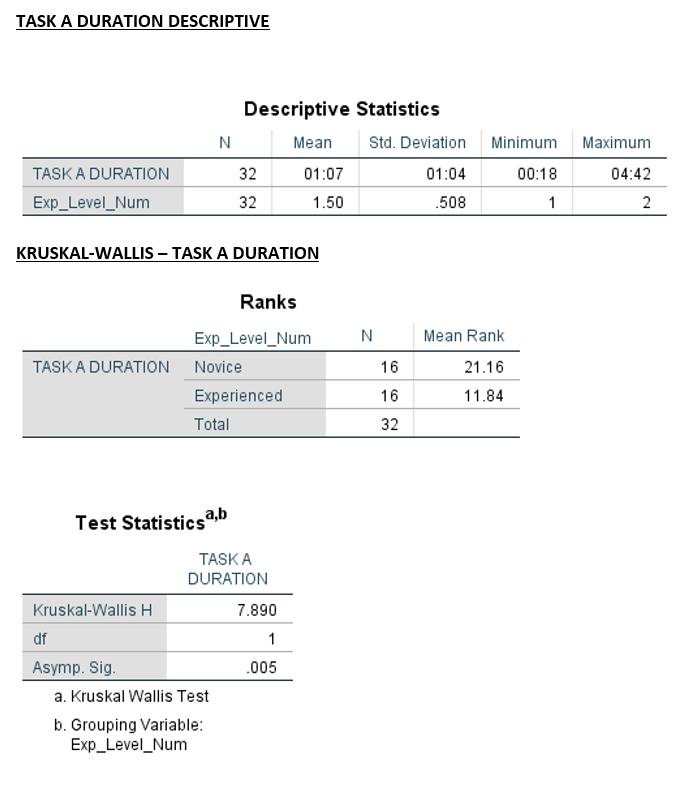
\includegraphics[width=\linewidth]{Screenshots/UXResearchDataFiles/UXTaskDurationData/taskDurationAStatsEdited.png}
%\label{DurationTaskA}
%\caption{Task A Duration Results}
%\end{table}

%\begin{table}[H]
%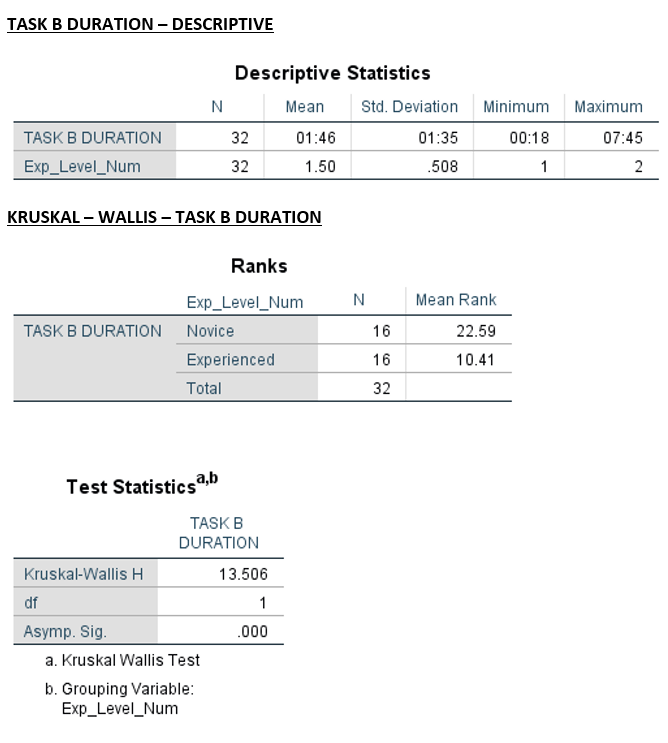
\includegraphics[width=\linewidth]{Screenshots/UXResearchDataFiles/UXTaskDurationData/taskDurationBStatsEdited.png}
%\label{DurationTaskB}
%\caption{Task B Duration Results}
%\end{table}

%\begin{table}[H]
%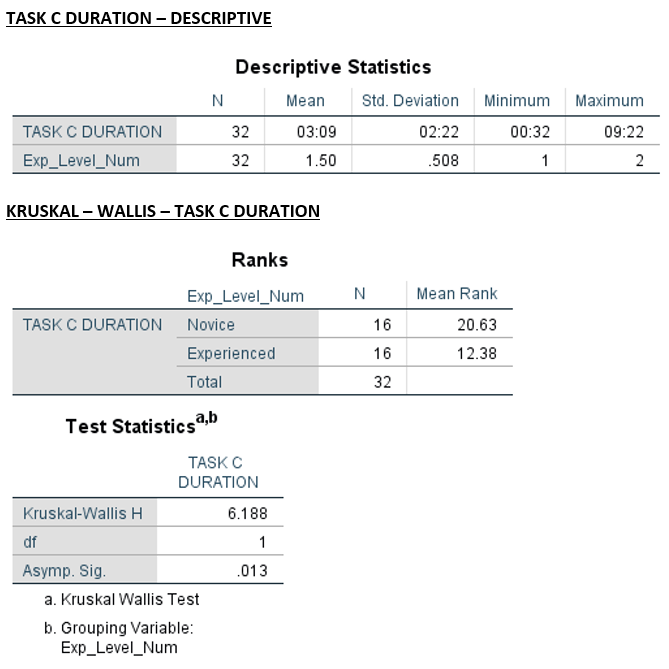
\includegraphics[width=\linewidth]{Screenshots/UXResearchDataFiles/UXTaskDurationData/taskDurationCStatsEdited.png}
%\label{DurationTaskC}
%\caption{Task C Duration Results}
%\end{table}

%\begin{table}[H]
%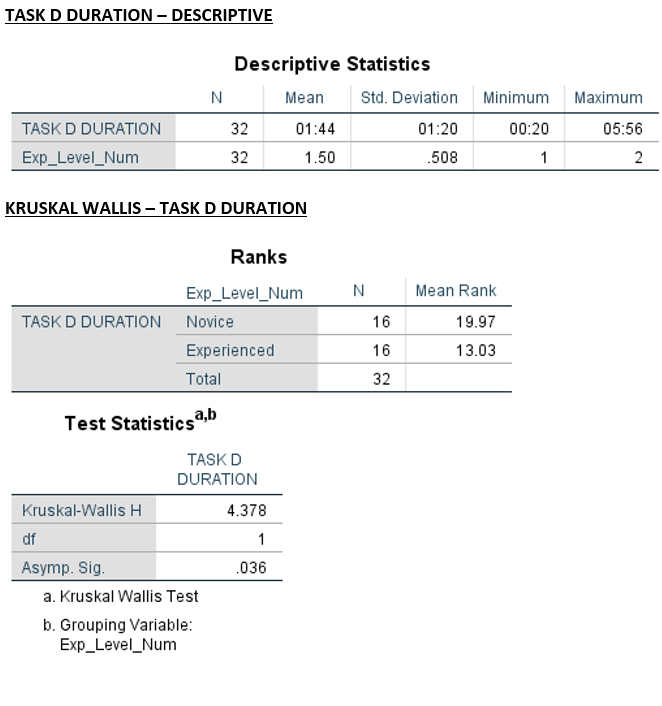
\includegraphics[width=\linewidth]{Screenshots/UXResearchDataFiles/UXTaskDurationData/taskDurationDStatsEdited.png}
%\label{DurationTaskD}
%\caption{Task D Duration Results}
%\end{table}

%\begin{table}[H]
%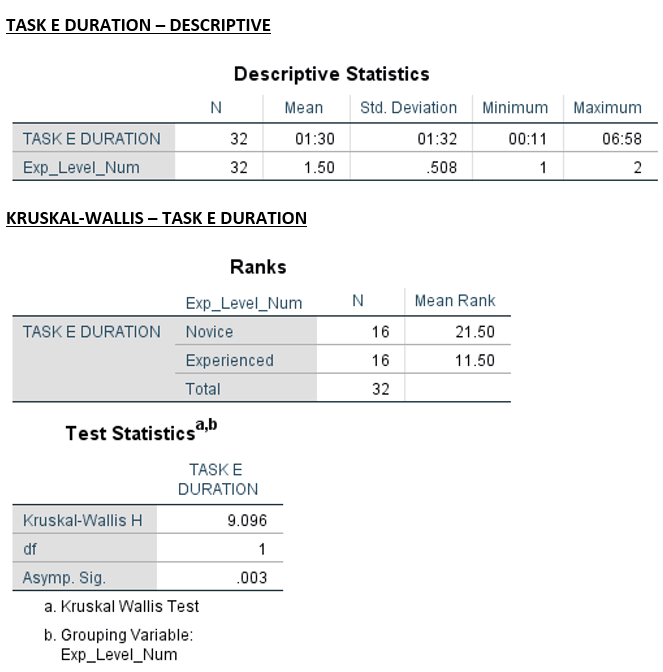
\includegraphics[width=\linewidth]{Screenshots/UXResearchDataFiles/UXTaskDurationData/taskDurationEStatsEdited.png}
%\label{DurationTaskE}
%\caption{Task E Duration Results}
%\end{table}

%\begin{table}[H]
%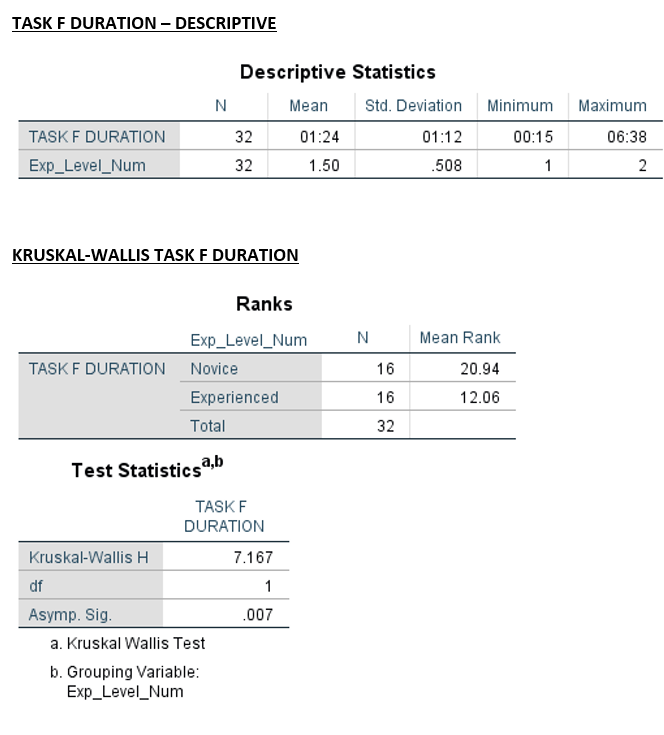
\includegraphics[width=\linewidth]{Screenshots/UXResearchDataFiles/UXTaskDurationData/taskDurationFStatsEdited.png}
%\label{DurationTaskF}
%\caption{Task F Duration Results}
%\end{table}

%\begin{table}[H]
%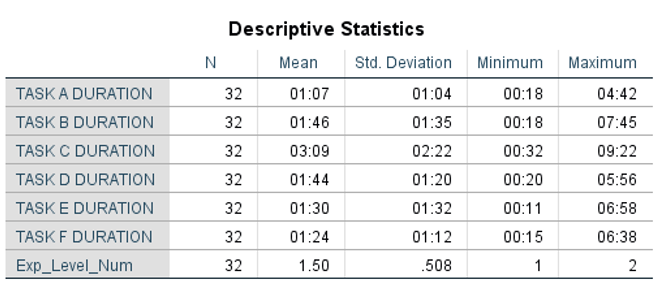
\includegraphics[width=\linewidth]{Screenshots/UXResearchDataFiles/UXTaskDurationData/taskDurationOverallStatsDescriptiveEdited.png}
%\label{DescriptiveDurationTotalPopulation}
%\caption{Task Duration Descriptive Statistics for Total Population}
%\end{table}

\begin{table}[H]
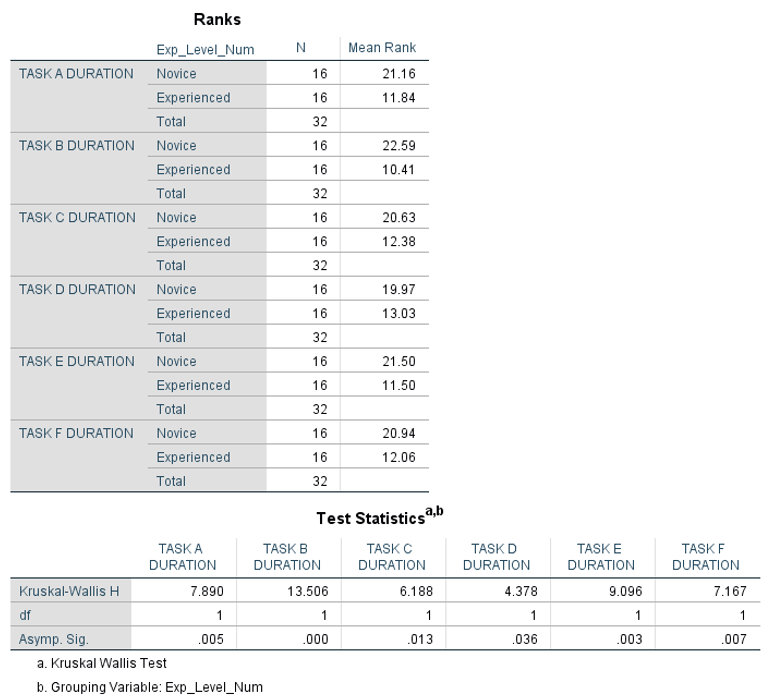
\includegraphics[width=\linewidth]{Screenshots/UXResearchDataFiles/UXTaskDurationData/taskDurationOverallStatsKWEdited.png}
\label{DescriptiveDurationTotalKW}
\caption{Task Duration Descriptive Statistics for Total Population}
\end{table}

This table shows all Task Duration data into one table, including the Mean rank that Novice and Experienced data sets hold, and more interestingly the Kruskal-Wallis examinations per task. Any task with an assumption signature equalling 0.05 or below indicates a significant difference between Novice and Experienced participants in the study. Much like with the participants encountering errors, the Novices have a higher Mean rank, thus demonstrating a greater amount of time spent in each Task compared to that of the Experienced participants. Regarding the Kruskal-Wallis assumption figures it is clear that Tasks A, B and E have the presence of significant differences between that of Novice and Experienced Users, especially with regards to Task B. Thus, Task C, D and F have no significant difference between those of Novice and the Experienced group. Task D shows the most similarity between the two types of user, with a assumption signature of 0.36, which corresponds to the proceed variance results, followed by Task C and F, although Task F almost reaches the threshold needed to be deemed significantly different. Therefore participants of both types interacted with Task C and D in a similar way in terms of how long they spent on each Task as well as Task F.


\section{Task Completion}
\begin{table}[H]
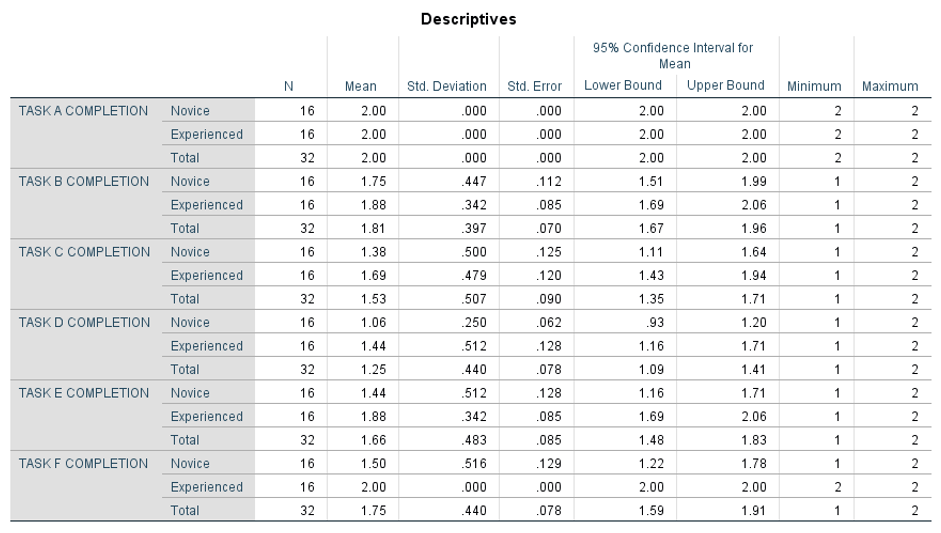
\includegraphics[width=\linewidth]{Screenshots/UXResearchDataFiles/UXTaskCompletionData/anovaDescriptivesTaskCompletion.png}
\label{DescriptiveTaskCompletionTotalPopulation}
\caption{Task Completion - Descriptive Statistics Novices and Experienced Participants}
\end{table}

As with Task Duration, Table 5.8 demonstrates several descriptive statistics analysed from both Novice and Experienced Participants. To determine whether a participant had completed a Task successfully or not, a scoring system was implemented. If a participant scored ``1" the Task was not completed successfully, whilst a score of ``2" meant that the participant completed the Task successfully, that is with the expected outcome. Task A was the only task to be successfully completed by participants of both categories with no participant failing to complete this Task, additionally all experienced participants successfully completed Task F, whereas several Novices were unable to do so. All other Tasks are more varied, but the generic trend showed that Novice participants were unable to complete more tasks compared with the Experienced participants. More detailed figures can be seen within Appendix A, Further Results.

%\begin{table}[H]
%includegraphics[width=\linewidth]{Screenshots/UXResearchDataFiles/UXTaskCompletionData/TaskACOMPLETIONEdited.png}
%\label{TaskCompletionA}
%\caption{Task A Completion Results}
%\end{table}

%\begin{table}[H]
%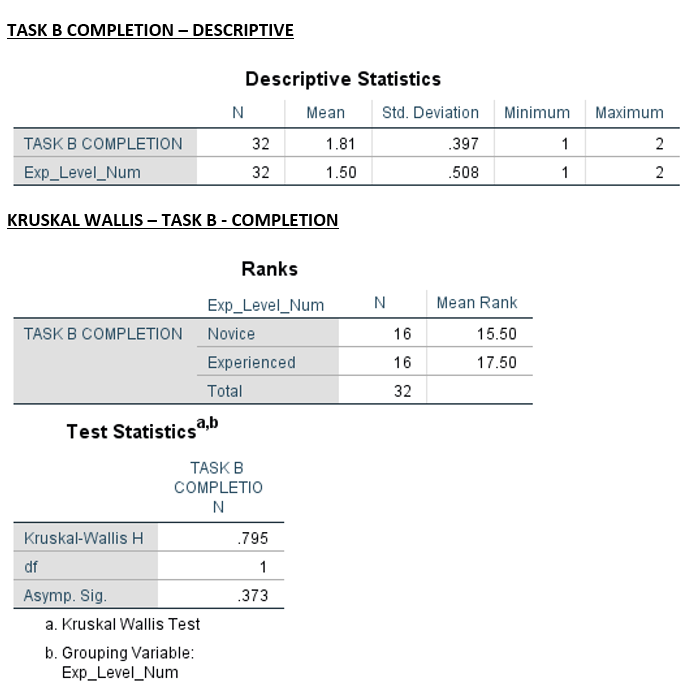
\includegraphics[width=\linewidth]{Screenshots/UXResearchDataFiles/UXTaskCompletionData/TaskBCOMPLETIONEdited.png}
%\label{TaskCompletionB}
%\caption{Task B Completion Results}
%\end{table}

%\begin{table}[H]
%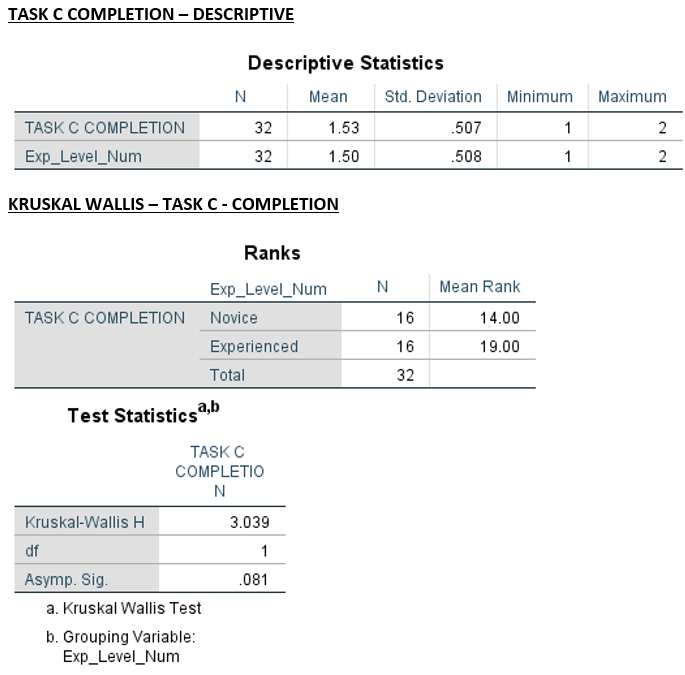
\includegraphics[width=\linewidth]{Screenshots/UXResearchDataFiles/UXTaskCompletionData/TaskCCOMPLETIONEdited.png}
%\label{TaskCompletionC}
%\caption{Task C Completion Results}
%\end{table}

%\begin{table}[H]
%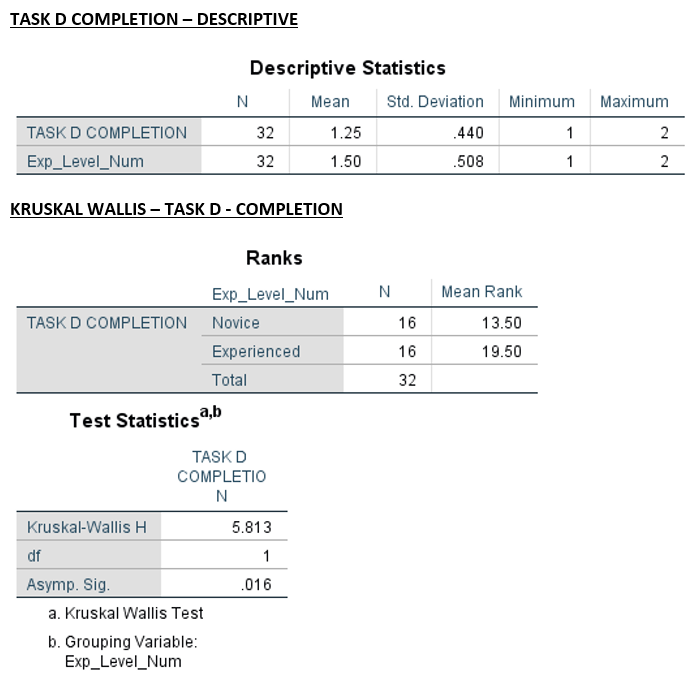
\includegraphics[width=\linewidth]{Screenshots/UXResearchDataFiles/UXTaskCompletionData/TaskDCOMPELTIONEdited.png}
%\label{TaskCompletionD}
%\caption{Task D Completion Results}
%\end{table}

%\begin{table}[H]
%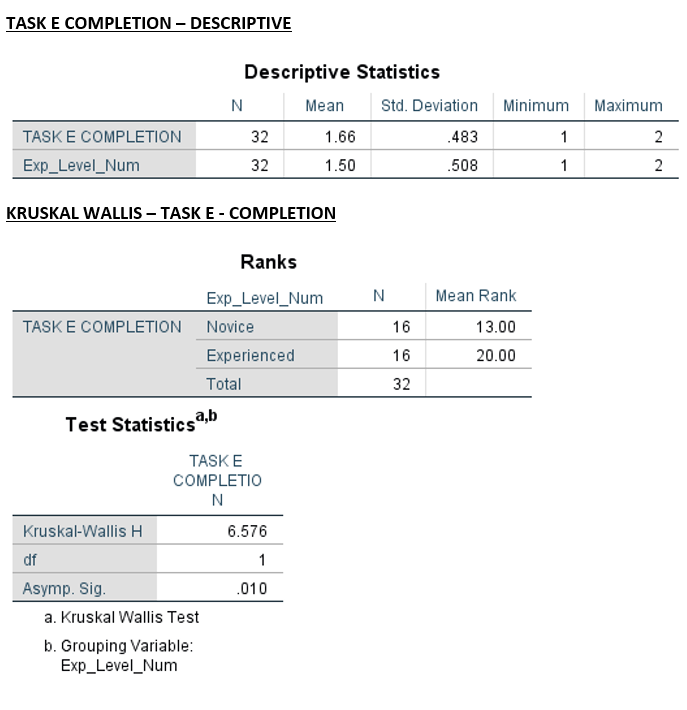
\includegraphics[width=\linewidth]{Screenshots/UXResearchDataFiles/UXTaskCompletionData/TaskECOMPLETIONEdited.png}
%\label{TaskCompletionE}
%\caption{Task E Completion Results}
%\end{table}

%\begin{table}[H]
%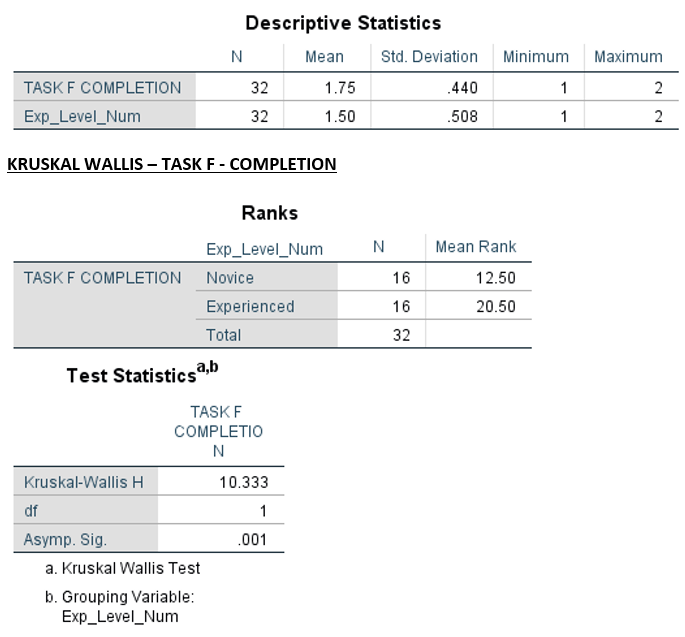
\includegraphics[width=\linewidth]{Screenshots/UXResearchDataFiles/UXTaskCompletionData/TaskFCOMPLETIONEdited.png}
%\label{TaskCompletionF}
%\caption{Task F Completion Results}
%\end{table}

\begin{table}[H]
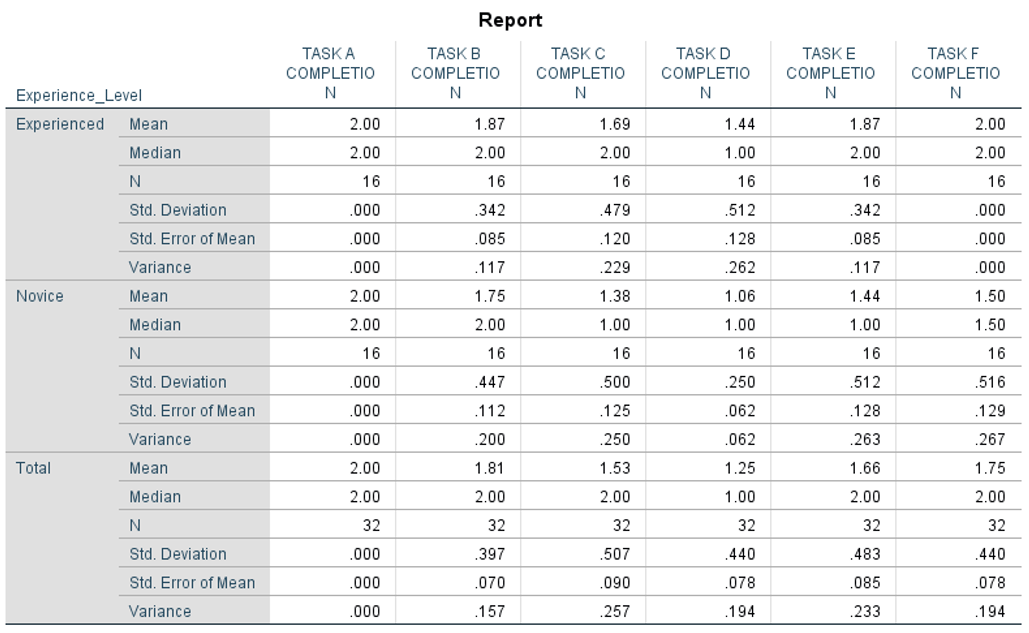
\includegraphics[width=\linewidth]{Screenshots/UXResearchDataFiles/UXTaskCompletionData/TaskCOMPLETIONOVERALLDESCRIPTIVEEdited.png}
\label{DescriptiveTaskCompletionAllTasks}
\caption{Task Completion - Further Descriptive Statistics for Total Population}
\end{table}

Novice and Experienced participants data sets show some variation, with the exception of the aforementioned Task A, where no differences were present between Novice and Experienced users. Task F showed the most variance in the Novice data set, with 50\% of participants completing the task successfully and the remaining failing to do so. Experienced participants show the most variance with Task D, with 43.8\% (7) of experienced participants completing the Task, with the remainder of 56.3\% (9) failing the task. Combining both data sets Task C showed the most variation, with 46.9\% (15) failing and 53.1\% (17) succeeding in completing the Task across both experience groups. 


\begin{table}[H]
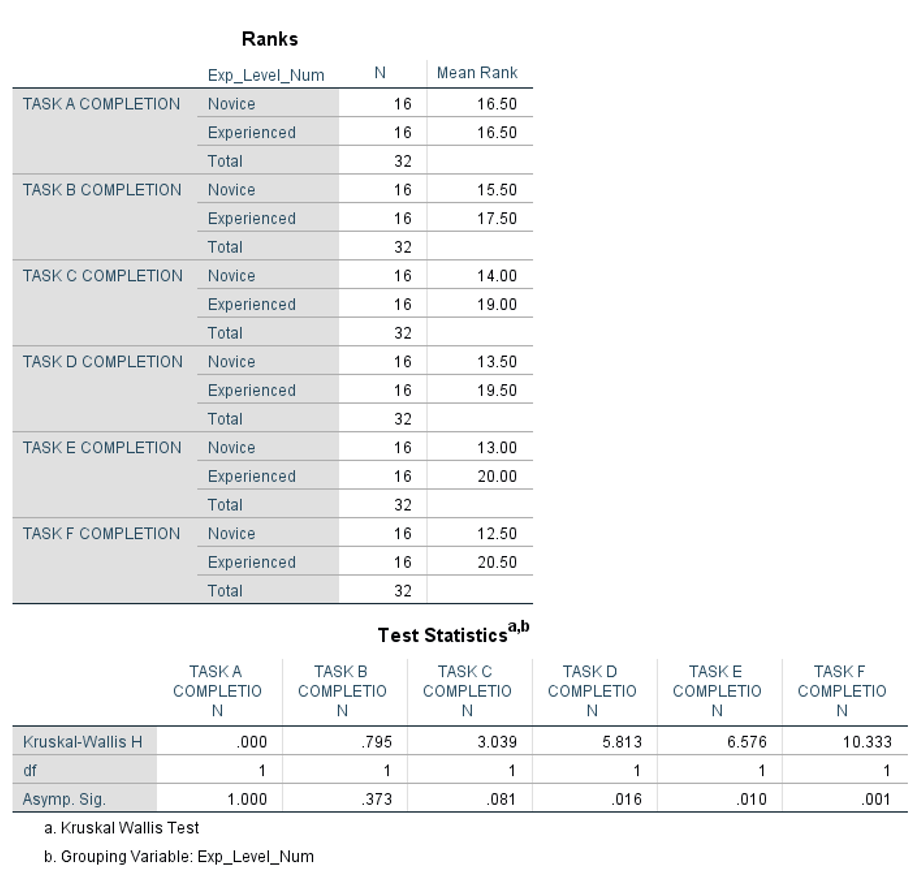
\includegraphics[width=\linewidth]{Screenshots/UXResearchDataFiles/UXTaskCompletionData/ALLTaskKWCompletionEdited.png}
\label{DescriptiveTaskCompletionALLKW}
\caption{Task Completion All Kruskal Wallis Results for all Tasks}
\end{table}

This table shows all previous Task Completion data into one table. According to the Kruskal-Wallis significance tests, Only Task F has a significant difference between that of Novice and Experienced Users, with a assumption figure of 0.01. All other tasks show no significant difference, with both Novice and Experienced users showing no difference in their completion of Task A, as all participants successfully completed the Task.

\section{Task Mouse Interactions}

\begin{table}[H]
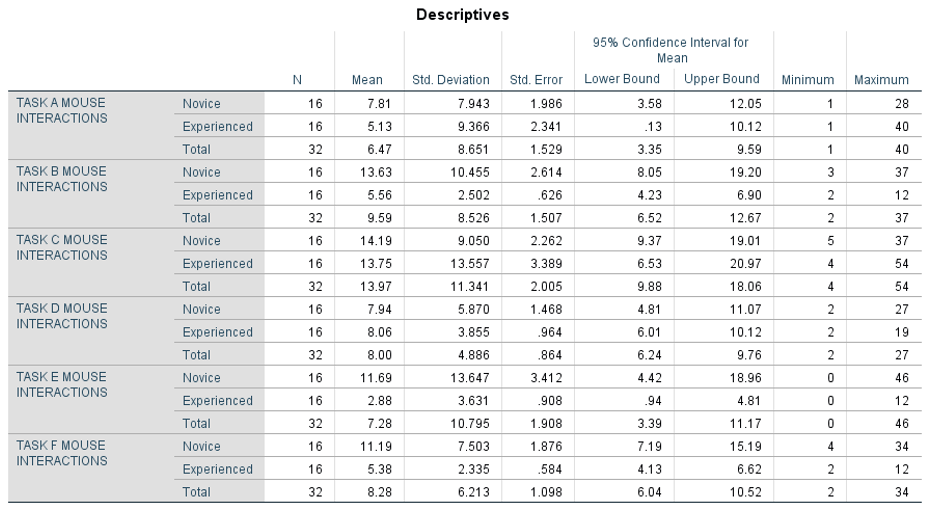
\includegraphics[width=\linewidth]{Screenshots/UXResearchDataFiles/UXTaskMouseInteractionsData/anovaDescriptivesTaskMouseInteractions.png}
\label{DescriptiveMouseInteractionsAllTasks}
\caption{Task Mouse Interactions Descriptive Statistics for Total Population}
\end{table}

As with all previous metrics Table 5.11 shows descriptive statistics taken from both Novice and Experienced participants data records of the number of Mouse Interactions made to attempt to complete each Task. As generally expected with the other other metrics collected, Novice participants overall took more mouse interactions when attempting each Task compared with their Experienced counterparts. Task C proved the most complex Task to attempt, with both Novice and Experienced participants using more mouse interactions within that Task. The maximum amount of mouse interactions made was also within Task C, with 54 clicks being recorded as the highest amount surprisingly by an Experienced participant. This participants score can be explained by the usage of the mouse provided during the experiment as the participant double clicked on each element interacted with, thus inflating their score twice as much as another participant who only single clicked on the majority of elements.

%\begin{table}[H]
%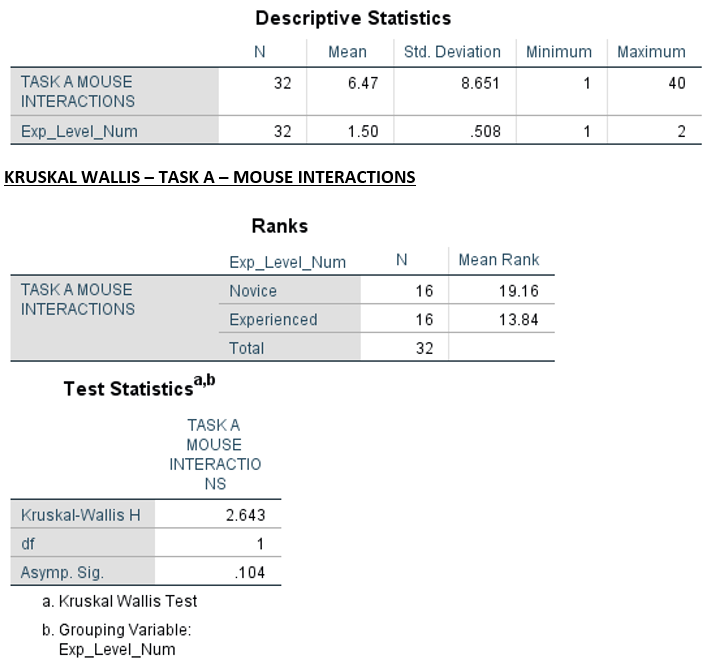
\includegraphics[width=\linewidth]{Screenshots/UXResearchDataFiles/UXTaskMouseInteractionsData/TaskAMouseInteractionsEdited.png}
%\label{TaskAMouseInteractions}
%\caption{Task A Mouse Interactions Results}
%\end{table}

%\begin{table}[H]
%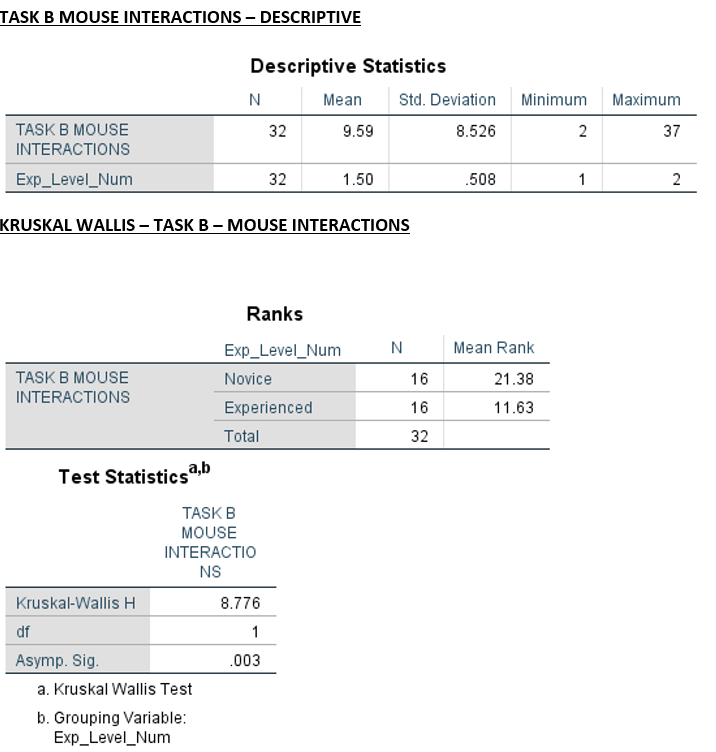
\includegraphics[width=\linewidth]{Screenshots/UXResearchDataFiles/UXTaskMouseInteractionsData/TaskBMouseInteractionsEdited.png}
%\label{TaskBMouseInteractions}
%\caption{Task B Mouse Interactions Results}
%\end{table}

%\begin{table}[H]
%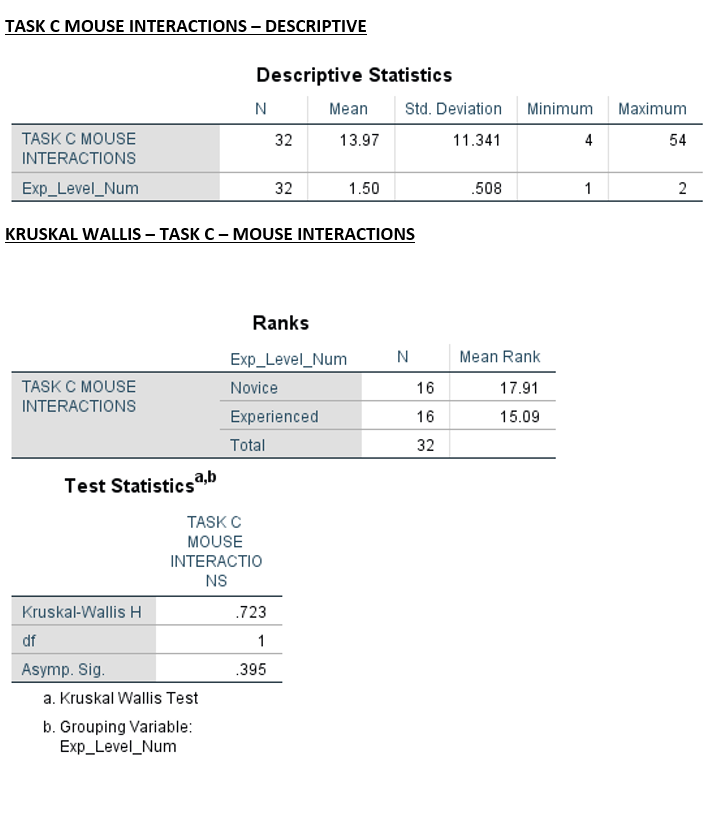
\includegraphics[width=\linewidth]{Screenshots/UXResearchDataFiles/UXTaskMouseInteractionsData/TaskCMouseInteractionsEdited.png}
%\label{TaskCMouseInteractions}
%\caption{Task C Mouse Interactions Results}
%\end{table}

%\begin{table}[H]
%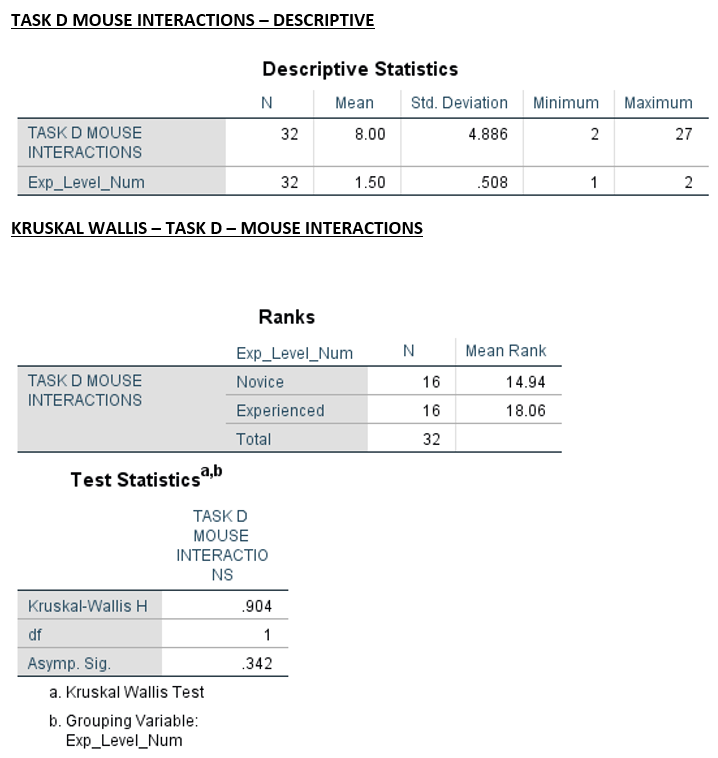
\includegraphics[width=\linewidth]{Screenshots/UXResearchDataFiles/UXTaskMouseInteractionsData/TaskDMouseInteractionsEdited.png}
%\label{TaskDMouseInteractions}
%\caption{Task D Mouse Interactions Results}
%\end{table}

%\begin{table}[H]
%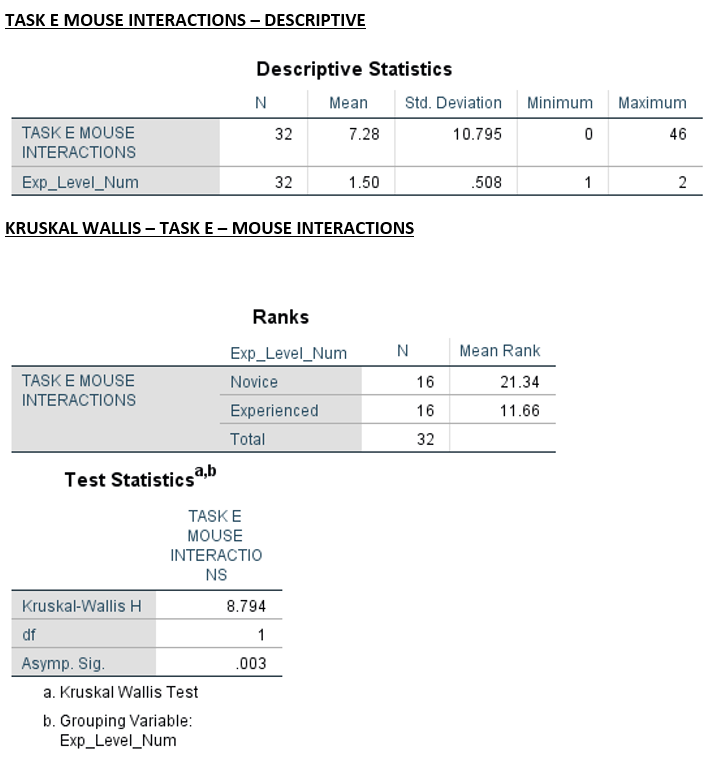
\includegraphics[width=\linewidth]{Screenshots/UXResearchDataFiles/UXTaskMouseInteractionsData/TaskEMouseInteractionsEdited.png}
%\label{TaskEMouseInteractions}
%\caption{Task E Mouse Interactions Results}
%\end{table}

%\begin{table}[H]
%\includegraphics[width=\linewidth]{Screenshots/UXResearchDataFiles/UXTaskMouseInteractionsData/TaskFMouseInteractionsEdited.png}
%\label{TaskFMouseInteractions}
%\caption{Task F Mouse Interactions Results}
%\end{table}

\begin{table}[H]
\includegraphics[width=\linewidth]{Screenshots/UXResearchDataFiles/UXTaskMouseInteractionsData/OverallDescriptiveTaskMouseInteractionsEdited.png}
\label{DescriptiveMouseInteractionsTotalPopulation}
\caption{Task Mouse Interactions Descriptive Statistics for Total Population}
\end{table}

Mouse interactions made by participants also show a notable amount of variance between Novice and Experienced participants. Novices show more variation in the amount of mouse interactions made between one another compared with internal comparison of experienced participants, with the exception of Task C, due to the inflation of one participants results, as described with Table 5.11. The highest level of variance shown within the novice data set is within Task E, with a maximum of 46 mouse interactions made by a Novice participant (See Table 5.11).

\begin{table}[H]
\includegraphics[width=\linewidth]{Screenshots/UXResearchDataFiles/UXTaskMouseInteractionsData/AllTasksMouseInteractionsKWEdited.png}
\label{AllMouseInteractionsKW}
\caption{Task Mouse Interactions All Kruskal Wallis Results for all Tasks}
\end{table}

Much like the previous two data metrics, this table shows all data sets for Task Mouse Interactions with the Mean rank and Kruskal-Wallis examination of the two data sets. The first Table, showing the Mean rank for the each of the Tasks shows that The majority of tasks show that Novices have a higher mean rank, with the exception of Task D. Task C is again notable for sharing a closely similar rank between the two groups. Task B, E and F show significant differences between that of Novice and Experienced groups, with these tasks all having an assumption figure of 0.05 or less. Therefore Task A, C and D do not have a significant difference between that of each experience group. This is to be expected, as has been seen with other data collected, Tasks C and D proved difficult for several of the participants regardless of experience category.

\chapter{Discussion}
\section{Overview}
The following section will discuss the results gained during the study that have been presented in Chapter 4 and Chapter 5, Participant Demographics and Research Results respectively. They will be discussed in the context of this projects aim, objectives and research questions that were presented in Chapter 1. The results will also be compared with previous studies as discussed within the literature review, especially those regarding the works investigating the roles of previous user experience, such as that of Dillon and Song's work with graphical element prompts and how Novice users interacted with them \citep*{dillon1997empirical}.

\section{Results Discussion}

\subsection{Issue and Error Detection}
The main aim of this project was to assess the impact that previous user experience has upon the Think-aloud methodology, within a concurrent testing environment. Therefore as part of this assessment between Novice and Experienced users I have collected extensive data on the amount and specific types of issues encountered by each type of participant, other metrics will be assessed in the sections following this one. Research Question One (RQ1) and Two (RQ2) can now be answered following this data collection and analysis. Types of errors encountered by both types of participant show overlap when regarding each experience sample as a collective. This was especially seen with Task C and D, as both types of users discovered the same exact issues, namely not being able to access required interface elements when attempting Task D, as the proprieties menu for the tested game ``Hollow Knight" was not obvious to the user regardless of their experience for the majority of participants. These results confirm other studies results using different programs, regarding the overlap of error types \citep{prumper1991errors}, which found Novice and Expert participants users to find the same types of errors whilst using a set of standard office tools. However, this research differs from previous studies as well, as in this study Novice and Expert found a different amount of issues and errors overall, with Novice users finding more issues compared with the Expert users, with thirty total issues detected compared with only eleven for Experienced participants. This difference has also been present in previous studies \citep{gerardo2007effectiveness}. Therefore with regards to Issues and Errors, the data in this study presents the fact that Novice and Experienced users show similarities in the errors that are detected, but also a great difference in the total number of errors detected overall, and the null hypothesis introduced in Chapter 1, must at least be partially rejected. Additionally, by having a smaller sample or less diverse sample size this would likely have led to a smaller amount of detected errors overall.

\subsection{Task Duration}
The next metric for discussion is the time it took both types of participant to complete each of the Tasks, known in this study as ``Task Duration" and was collected for each Task individually. Therefore Research Question Three (RQ3) can now be analysed. As highlighted in Chapter 5, some of the six tasks showed significant differences between Novice and Experienced users. Task C had the most time spent for both Novice and Experienced users, which was expected as Task C was designed to be the most complex Task. Novice, Experienced and combined user data sets show a great difference in variation between the different Tasks (see Table 5.6). Experienced users had a tighter grouping of variance amongst the sixteen participants, as compared with Novices which showed greater variance, that is with the exception of Task C, as both groups share a significant level of variation in that Task. Task D showed less variation for Novice results compared with the Experienced participants, meaning that more Novice users took a similar amount of time (which was longer than that of Experienced users). As presented in Table 5.7, Kruskal-Wallis examinations show that Task A, B and E show a significant level of difference in Novice and Experienced participants data sets. Therefore half of the Tasks show what a significant difference previous user experience makes upon how long Tasks are completed or attempted. The fact that these Tasks show this significant could be indicative of problems within the Steam client, but crucially shows that Concurrent Think-aloud testing will be impacted by a participants level of experience regarding Task Duration. Novices are likely to take longer to complete tasks at least in 50\% of tested cases. Therefore, regarding Research Question Three, there is the presence of a discrepancy within this study between the tested experience groups.

\subsection{Task Completion}
Task Completion was also assessed within this study, if a Task had a high failure rate, it would be potentially indicative of a problem within the tested service or problems with the description or structure of the study. Some of the tasks show high failure rates within this study, as well as consistent successful Tasks between the types of participant, and as such Research Question Four can now be assessed. Overall Task D was the most difficult Task, for both Novice and Experienced users, holding a failure rate of 75\% when considering all 32 participants in both categories combined, the reason for this was likely twofold. Firstly, this tasks interface hidden from the user, requiring knowledge on how to access games properties menu, and thus is a significant design issue within the Steam interface. Secondly, the word ``Verification" confused many of my participants as they did not understand what that meant in regards to game services, this was especially true of my Novice participants as many would verbally explain their confusion. Therefore this study has uncovered a problem regarding the way in which Tasks a presented to participants, an observation seen in other works prior to this \citep{gerardo2007effectiveness}; but also uncovered the tested service design faults at least 4 Tasks. On an individual level, Task C showed a significant number of Novice participants failing the Task, alongside Task E and F. Whereas Task C was only failed by 5 experienced participants (31.3\%). Task F is shows significant differences between Novice and Experienced groups following the Kruskal-Wallis test. However according to Kruskal-Wallis examinations of the Novice and Experienced data sets, only Task F shows a significant difference of success or fail ratio in Task Completion, with only eight Novice participants successfully completing the Task, compared with all sixteen Experienced participants completing Task F. Therefore Research Question Four can be answered by saying that in the majority of cases experienced users are more likely to have a higher completion success rate, compared with Novice users when tasks are regarding more complex functions. However in the case of Task A, functions which are similar to other services such as database records or shopping websites such as Amazon.com, lead to close or exact similarity between Novice and Experienced participants. There is also no significant difference between the data sets according to the Kruskal-Wallis test, except with Task F.

\subsection{Task Mouse Interactions}
Additionally this study also included the collection of the number of Mouse Interactions per Task which is not commonly seen in other studies similar to this work. Mouse Interactions were defined as how many clicks of the mouse were made whilst attempting or completing each Task. Therefore Research Question Five can now be examined. As with the other metrics recorded in this project, a higher amount of mouse interactions could again be indicative of a design problem within the tested service, as a large amount of clicks could mean that participants are unsure of how the tested interface is supposed to work. For the majority of Tasks, Novice users clicked more times during their attempts as compared with Experienced participants. The former statement is true for the mean Mouse interactions made for each Task except with Task D. Interestingly, Task C shows that Novice and Experienced users were extremely similar in their use of the program regarding Mouse interactions (see Table 5.11). Mouse Interactions also show some variation between Novice and Experienced data sets, again showing that Novice users are more varied in their approach to using Steam, and experienced participants are less so, taking a similar amount of Mouse interactions with all tasks with the exception of Task C, where the inverse of this true and Novice users are more consistent in the numbers of Interactions made in that Task. The Kruskal Wallis examination of Mouse Interactions Data do show some significant differences between the two groups, but only in 50\% of tasks, Task B, E and F, much like with Task Duration which showed significant differences in three Tasks (Tasks A, B and E). Therefore to answer Research Question Five, Novice and Experienced users do show significant differences in the number of Mouse Interactions made in 50\% of tasks, but not for the remainder of tasks.

\subsection{Participant Post Questionnaire}
Lastly, participants were asked for their thoughts on their involvement in this study. Firstly participants were asked for their thoughts on the Steam services usability and secondly their ratings of Thinking-aloud and whether or not that distracted them during the study, and as such Research Question 6 can now be answered. Before the collection of the results, the expectation was that Novice users would find the Steam service more difficult and less user friendly compared to the experienced participants who were used to gaming services from other platforms.  This proved to be the case for the majority of Novice participants as seen in Figure 4.13 as most participants rated the service in the D or E category, elaborating that visual elements were complex, cluttered or obscure, this coupled with problems with understanding aspects of gaming showed both a higher amount of issues (as discussed above) and thus lead to this assessment of the Steam interface in terms of its interface. Conversely the majority of Experienced participants commented on the services relative ease of use and lacking problems in functionality, except when commenting on Task D, as the properties menu for games is hidden and not very intuitive. However when asked about the Think-aloud process their is no significant difference in what each experience group commented on, as both groups responded favourably to Thinking-aloud and that for the most part they did not find it to interfere with there use of the program. Thus to answer Research Question 6, it can be stated that participants react to the Think-Aloud process similarly regardless of previous user knowledge, However they do react differently when asked about the overall usability of the tested service. 


\section{Summary}
This chapter has discussed the results of the study as seen in Chapter 4 (Participant Demographics) and Chapter 5 (Research Results). There have been striking differences between Novice and Experienced participants in these different metrics especially regarding tasks C, D and F, but also some unexpected similarities regarding some Tasks which was not anticipated prior to this study. These results have also been compared with previous works.  








\chapter{Recommendations for the Steam Service}
\section{Overview}
Although this project has the main aim of assessing the impact of previous user knowledge on the Concurrent \gls{ta} methodology, as part of this process a series of issues have been uncovered by both Novice and Experienced participants alike, with significant overlap between the groups (see section \ref{NoviceErrorsList} and section \ref{ExperiencedErrorsList}). Therefore this chapter will discuss the most common issues encountered in this study regardless of type of participant, before suggesting some potential solutions that could be implemented to help alleviate this issues with the Steam Client, although this tested version of the software is in the process of being updated \citep{pcGamerSteamUI2019}.

\section{Most Common Issues}
\begin{itemize}
    \item Visual Layout -  cluttered elements
    \item Hidden Functions
\end{itemize}

\section{Potential Remedies}
\begin{itemize}
    \item Simplification or removal of elements that are not commonly used
    \item Colour palette update - increase brightness of software as many elements are not seen initially due to black visuals.
    \item make help section more obvious
\end{itemize}


\chapter{Conclusion}

\section{Overview}
This final chapter will collate all previously discussed results and assess what this research has provided to the academic community within \gls{ux} research. The projects aims and objectives will then be assessed. Lastly the projects limitations and any suggestions for future work shall be discussed.

\section{Project Conclusions}
The main aim of this project was to assess the influence that previous user knowledge has upon the Concurrent Think-Aloud methodology. Therefore a Concurrent Think-Aloud study using PC gaming service Steam made by the Valve Corporation was conducted. A total of thirty-two participants were involved split into two equal groups, Novice and Experienced. These participants were asked to attempt six tasks within the Steam client, which encompassed many of the common functions used in the program, such as searching the Store for purchasable games or changing the \gls{ui} for a more console like experience. When each of this tasks were attempted, several data metrics were collected. This metrics included Task Duration, Task Completion, Task Mouse Interactions, Reception to the Think-Aloud Protocol, Usability Assessment of the Steam service, and crucially the frequency and types of issues or errors encountered in the test process. Each participant experienced similar conditions, regarding environment and the equipment used in the testing. This data was then organised using Microsoft Excel and analysed using SPSS.

The results revealed that Novice and Experienced participants do have show significant differences in regard to some Tasks, especially those which are more complex, which in this study was Task C and D and therefore Experienced participants are more efficient at using services, but in this study found less issues overall. This is likely because Steam is a highly developed software which has been on the market since 2004. However several similarities were also present between the two types of participant. Firstly, some of the same issues were detected by both participants, which some studies have suggested is not the case. Additionally both types responded similarly when asked about Thinking-aloud. Lastly, Novice and Experienced participants react similarly to certain tasks, as has been seen in Task A, where all participants where able to complete the Task successfully. 

\section{Project Objectives and Aim Evaluation}

This section will now evaluate the success project via an assessment of the Objectives and overall project Aim. The first objective was \textit{to review and discuss relevant literature around issues of usability and the Think-Aloud Methodology}. This objective was met in Chapter 2 - Literature Review, as discussion surrounding the field of usability testing and more specific works regarding the use and assessment of previous user experience in past studies is present. The second objective was \textit{to arrange and execute a Think-Aloud usability study with the expectation of 40 participants split across two categories of Novice and Experienced users, using the game distribution service Steam}. This has been achieved, as evidenced by the multiple chapters, especially chapters 4 and 5 which present the results of this study. The next objective was \textit{to provide critical analysis of collected data from Novice and Experienced participants and draw conclusions on any significant outcomes}, this objective has been completed as evidenced by Chapter 6 - Discussion, which deduces several findings based on the analysed data sets. Lastly the final objective was \textit{to provide suitable feedback based on the outcome of the study to the Valve corporation to improve the Steam service}, although this objective is secondary, it still has been met in Chapter 7 - Recommendations for the Steam service,  which discusses some theoretical options for improvements of the Steam software. Therefore all Objectives can be considered met, and thus the Aim of the project also.

\section{Limitations}
During the process of conducting this project I have encountered several limitations and problems that should be addressed, should this projects work be expanded upon in the future. The largest set of limitations revolves around the Demographics of the Experienced participants compared against the make-up of the Novice sample. The majority of participants in the Experienced category were aged between 18-30 and were male, with only three female participants out of sixteen. Conversely the Novice category had a more balanced set of demographics with an equal amount of male and female participants, and a greater range of participant ages. A general flaw from this project also included the fact that the intention of having forty participants split into twenty Novices and twenty Experienced participants was not realised, with only thirty-two participants (16 Novices, 16 Experienced) thus having 8 missing participants that were expected.  The second aspect that could be expanded upon is the Task list itself. The six tasks tested the most commonly used functions of the Steam interface. However other aspects were not examined. For instance, Steam offers a service were users can purchase and trade in game items usually cosmetic in nature, known as the Steam Marketplace, a task could be based upon this, however if too many Tasks are present then a participant may become tired and behave differently than when they first started the test. Thirdly, this project also uncovered issues encountered with the terminology used within the Tasks, especially when they were attempted by the Novice participants, this was seen in the word verification Task D, and Big Picture Mode in task E.

\section{Suggestion for Further Work}
With the conclusion of this project, there are various aspects that could be expanded upon in future works. Firstly, as mentioned above this sample had the expectation of forty participants, however future studies could have a larger pool of participants compared to this, perhaps in the hundreds. However this would be very time consuming and potentially not beneficial to researchers or specific tested platforms. Additionally any future work could involve more specialised forms of knowledge experience groups such as Novice, Experienced, Expert. (Faulkner and Wick 2005). A greater and more diverse set of participants could have led to a greater amount of issues detected, as compared with this study results. Regarding the data collection phrase of the research, OBS and WhatPulse were used to record a visual record and count the numbers of Mouse interactions per tasks. However one such feature that could have been used in this study was the use of Heat maps, these heat maps could have been used on a Task by Task basis as well as overall usage of the Steam software. These heat maps would have shown the distribution of the areas of interactions, which adds another layer of metrics to this study, as well as pinpointing visually the most commonly used areas of Steam, and what areas are less frequently interacted with.
As already discussed in section 8.2, Steam is a mature piece of software, which has undergone a large amount of changes over its lifetime and as such issues encountered within the program are likely fewer than a newer piece of software or even an incomplete program or website. Additionally this study assessed the impact of previous user knowledge on the Concurrent-Think Aloud methodology, however as highlighted by Chapter 2 other Think-aloud methods exist and as such another study could be made involving these methods, especially Retrospective Think-aloud testing, during which I suspect that Novice users would react differently to that of Concurrent.

\section{Summary}
This research has tried to provide detailed assessment of the impact that Novice and Experienced participants have upon Concurrent usability testing, alongside this studies limitations and suggestions for further work in the evaluation of previous user experience in the testing of applications.  

% ------------------------------------------------------------------------
\nocite{*}
\setlinespacing{1.44}
%\bibliographystyle{amsplain}
\bibliographystyle{apalike}
\bibliography{XBib.bib}

%#### Include any appendix below #####
\begin{appendices}
\chapter{Further Research Results}
\section{Task Completion}
\begin{figure}[H]
\includegraphics[height=16cm]{Screenshots/UXResearchDataFiles/UXTaskCompletionData/novicePercentageCompletion.png}
\caption{Novice Task Completion Percentages}	
\end{figure}

\begin{figure}[H]
\includegraphics[]{Screenshots/UXResearchDataFiles/UXTaskCompletionData/experiencedPercentageCompletion.png}
\caption{Experienced Task Completion Percentages}	
\end{figure}




\chapter{Steam Software User Interface and Task Explanation}
\section{Figures associated with the Steam Store}
\begin{figure}[H]
\includegraphics[width=16cm,height=9cm]{Screenshots/SteamScreenShots/SteamMainShopMenu.png}
\caption{Steam Client Store Menu}	
\end{figure}
This is the default page for Steam and what would greet the user upon logging in. It displays the available games for purchase, with sub-categories available from the left hand side. There are a great number of interactive elements on this screen, so it may take some time for study participants to find exactly what they are looking for.

\begin{figure}[H]
\includegraphics[width=16cm,height=9cm]{Screenshots/SteamScreenShots/SearchingForAGame.png}
\caption{Searching for a title "DIRT 2.0" on the Steam Store Page}
\end{figure}
The above Figure demonstrates the basic search functionality of the Steam Store, where a user would type in the name of a specific game, or secondly an associated word such as a games publisher like "Codemasters" for the "Dirt Rally" franchise. Upon clicking a certain title, a page similar to Figure 4 shall appear.

\begin{figure}[H]
\includegraphics[width=16cm,height=9cm]{Screenshots/SteamScreenShots/PageForSearchedGameDirt.png}
\caption{Store Page for Searched Title - ``DIRT Rally 2.0"}    
\end{figure}
This page shows information about the searched title "DIRT Rally 2.0", the user can view the games description, any media such as video trailers and screen-shots from the game, they can choose to purchase the game, view overall community reception to the game, among other functions.

\section{Figures associated with the Steam Library - Installing a Game}
\begin{figure}[H]
\includegraphics[width=16cm,height=9cm]{Screenshots/SteamScreenShots/SelectAPurchasedGame.png}
\caption{Selection of ``Sid Meier's Civilization 5" in the purchased Library of Games}    
\end{figure}
This is the Steam library page, on the left hand side are a series of game titles belonging to my account. To install a title, a user would right click the desired game, and then follow the dialog box then is displayed in Figure 6.

\begin{figure}[H]
\includegraphics[width=16cm,height=9cm]{Screenshots/SteamScreenShots/InstallDialogForCivilisation5.png}
\caption{Installation Dialog Message Box - Sid Meier's Civilization 5}    
\end{figure}
The dialog box gives users information on what game they are installing and data such as installation size and the set file path. 

\section{Figures associated with Steam Community Modifications of Sid Meier's Civilization 5}

\begin{figure}[H]
\includegraphics[width=16cm,height=9cm]{Screenshots/SteamScreenShots/CommunityForCivilisation5.png}
\caption{Community Section for Sid Meier's Civilization 5}    
\end{figure}

This is the community section of the Steam client, it is used for a number of functions, including that of finding modifications for certain games, such as Sid Meier's Civilization 5. The user can find modifications suited to what they want to change, for instance music or graphical elements. For ease of use, many users would be interested in the most popular mods, which this UI offers as a shortcut seen at the centre - bottom of the image. 

\begin{figure}[H]
\includegraphics[width=16cm,height=9cm]{Screenshots/SteamScreenShots/FindingAModForCivilisation5.png}
\caption{Finding a Modification for Sid Meier's Civilization 5}    
\end{figure}

Once the user has clicked on the "Most Subscribed" element, a list of the most popular modifications is presented for the user to browse.

\begin{figure}[H]
\includegraphics[width=16cm,height=9cm]{Screenshots/SteamScreenShots/SubscribingToSelectedMod.png}
\caption{Subscribing to the R.E.D Modpack for Sid Meier's Civilization 5}    
\end{figure}

Upon clicking a particular modification of interest, the user is brought to a page detailing what the mod is, and the ability to ``subscribe to the mod". 

\section{Figures associated with verifying an installed game}

\begin{figure}[H]
\includegraphics[width=16cm,height=9cm]{Screenshots/SteamScreenShots/verifyCSProperties.png}
\caption{Opening a selected game properties menu from Steam Library page}    
\end{figure} 

This Figure shows an installed game ``Counter-Strike Global Offensive", I have right clicked on the white text to bring up a new menu, I am about to click on properties to bring up further options for this particular game.

\begin{figure}[H]
\includegraphics[width=16cm,height=9cm]{Screenshots/SteamScreenShots/verifyCSButtonLocation.png}
\caption{Locating the Verification of game files button for Counter-Strike : Global Offensive}    
\end{figure} 

I have located the required button to verify the game installed game files for Counter Strike : Global Offensive , \textit{``Verify Integrity of Game Files"}. 

\begin{figure}[H]
\includegraphics[width=16cm,height=9cm]{Screenshots/SteamScreenShots/verifyProcess.png}
\caption{Locating the Verification of game files button for Counter-Strike : Global Offensive}    
\end{figure}

I have clicked upon the desired button element, and the verification process has begun.

\section{Figures associated with the Big Picture Mode}
\begin{figure}[H]
\includegraphics[width=16cm,height=9cm]{Screenshots/SteamScreenShots/BigPictureModeTopRightCropped.png}
\caption{Location of Steams Big Picture Mode}    
\end{figure} 

This image, although similar to the image in Figure 2. This image focuses on the location of the UI element to change the Steam interface into big picture mode, it is located at the top right hand side of the client, near the user-name and user picture. It is indicated by a white rectangle with arrows. The interface will change to what is pictured in Figure 10, upon clicking the box.

\begin{figure}[H]
\includegraphics[width=16cm,height=9cm]{Screenshots/SteamScreenShots/SteamInBigPictureMode.png}
\caption{Big Picture Mode Enabled in the Steam Client}    
\end{figure}
This image shows how the Steam client is presented when in ``Big Picture Mode", which is a complete UI redesign suited for users who prefer using a controller over that of using mouse and keyboard.

\section{Figures associated with adding another user as a friend on Steam}

\begin{figure}[H]
\includegraphics[width=16cm,height=9cm]{Screenshots/SteamScreenShots/friendsUI.png}
\caption{Friends UI element of the Steam client}    
\end{figure}

The Steam client has a convenient function to display the accounts friends. The user is pictured in this Figure and shows currently added friends, who are online and offline as well as what friends are playing.

\begin{figure}[H]
\includegraphics[width=16cm,height=9cm]{Screenshots/SteamScreenShots/searchforAFriend.png}
\caption{Searching for a fellow Steam user to add them as a friend}    
\end{figure}

I have clicked on the small icon of a user with a plus arrow in the previous Figure UI, and am now presented with the following screen, I will search for a user ``Geogen", in the appropriate location.

\begin{figure}[H]
\includegraphics[width=16cm,height=9cm]{Screenshots/SteamScreenShots/friendRequestSent.png}
\caption{Sending a friend request to a desired user}    
\end{figure}

Following the previous Figure I have found a list of users with that name, the top user is the account I wish to add, so I have clicked the corresponding element (\textit{``ADD AS FRIEND"}) to send them a friend request.


\chapter{Project Materials}
\section{Study Invitation}
\begin{figure}[H]
    \includegraphics[width=14cm,height=16cm]{Screenshots/StudyMaterialScreenshots/Invitation.png}
    \caption{Study Invitation for Participants}
\end{figure}

\section{Study Information}
\begin{figure}[H]
    \includegraphics[width=16cm,height=22cm]{Screenshots/StudyMaterialScreenshots/informationPT1.png}
    \caption{Study Information for Participants}
\end{figure}

\begin{figure}[H]
    \includegraphics[width=16cm,height=22cm]{Screenshots/StudyMaterialScreenshots/informationPT2.png}
\end{figure}


\section{Pre-Study Questionnaire}
\begin{figure}[H]
    \includegraphics[width=16cm,height=22cm]{Screenshots/StudyMaterialScreenshots/preStudyQuestionairePT1.png}
    \caption{Pre-Study Questionaire for Participants}
\end{figure}

\begin{figure}[H]
    \includegraphics[width=16cm,height=22cm]{Screenshots/StudyMaterialScreenshots/preStudyQuestionairePT2.png}
\end{figure}

\begin{figure}[H]
    \includegraphics[width=16cm,height=22cm]{Screenshots/StudyMaterialScreenshots/preStudyQuestionairePT3.png}
\end{figure}

\section{Post-Study Questionnaire}
\begin{figure}[H]
    \includegraphics[width=16cm,height=24cm]{Screenshots/StudyMaterialScreenshots/postStudyQuestionaire.png}
    \caption{Post Study Questionnaire for Participants}
\end{figure}

\section{Consent Form for Participants}
\begin{figure}[H]
    \includegraphics[width=16cm,height=22cm]{Screenshots/StudyMaterialScreenshots/consentForm.png}
    \caption{Consent Form for Participants}
\end{figure}

\section{Participant Task List Instructions}
\begin{figure}[H]
\includegraphics[width=16cm,height=22cm]{Screenshots/StudyMaterialScreenshots/taskForParticipants.png}
\caption{Tested Steam Task List for Participants}
\end{figure}

\section{Task List For Study Practitioner}
\begin{figure}[H]
\includegraphics[width=16cm,height=22cm]{Screenshots/StudyMaterialScreenshots/tasklistPractioners.png}
\caption{Task List for Usability Study Practitioner}
\end{figure}

\section{Study Observation Sheet}
\begin{figure}[H]
\includegraphics[width=16cm,height=22cm]{Screenshots/StudyMaterialScreenshots/observationSheet.png}
\caption{Study Observation Sheet for Usability Study Practitioner}
\end{figure}

\section{Record Issue Sheet}
\begin{figure}[H]
\includegraphics[width=16cm,height=22cm]{Screenshots/StudyMaterialScreenshots/issuesEncounteredinStudy.png}
\caption{Record Issue Sheet for Usability Study Practitioner}
\end{figure}

\section{Study Procedure Task List}
\begin{figure}[H]
\includegraphics[width=16cm,height=22cm]{Screenshots/StudyMaterialScreenshots/studyProcedureList.png}
\caption{Study Procedure Instructions for Usability Study Practitioner}
\end{figure}

% =================================================================
\end{appendices}
\end{document}
% ------------------------------------------------------------------------
